\documentclass[10pt,twocolumn]{article}

% ── Packages ──────────────────────────────────────────────────────────────────
\usepackage[utf8]{inputenc}
\usepackage[T1]{fontenc}
\usepackage[margin=1in]{geometry}
\usepackage{amsmath,amssymb,amsthm}
\usepackage{graphicx}
\usepackage{booktabs}
\usepackage{hyperref}
\usepackage{xcolor}
\usepackage[expansion=false]{microtype}
\usepackage{caption}
\usepackage{subcaption}
\usepackage{natbib}
\usepackage{enumitem}
\usepackage{multirow}
\usepackage{array}
\usepackage{nicefrac}
% placeins.sty is not installed in this TeX Live tree and cannot be added
% without write access to the system texmf tree; \clearpage is a strictly
% correct (if less space-efficient than placeins's real barrier) substitute
% that guarantees every pending float is flushed before it fires.
\newcommand{\FloatBarrier}{\clearpage}

% ── Theorem environments ───────────────────────────────────────────────────────
\newtheorem{proposition}{Proposition}
\newtheorem{remark}{Remark}
\newtheorem{definition}{Definition}

% ── Colors ────────────────────────────────────────────────────────────────────
\definecolor{darkblue}{RGB}{13,49,114}
\definecolor{darkred}{RGB}{150,20,20}
\definecolor{darkgreen}{RGB}{20,100,40}
\hypersetup{colorlinks=true, linkcolor=darkblue, citecolor=darkgreen,
            urlcolor=darkblue}

% ── Column separator ──────────────────────────────────────────────────────────
\setlength{\columnsep}{0.25in}

% ── Title ─────────────────────────────────────────────────────────────────────
\title{\textbf{A Loose Ceiling, Not a Certificate: Auditing Fisher-Separability\\
Bounds on Hallucination Detectability Across Architectures\\
\large{(with Wasserstein Geometry and Conformal Guarantees)}}}

\author{
  Lakshmi Chakradhar Vijayarao \\
  Independent Researcher \\
  \texttt{lakshmichakradhar.v@gmail.com}
}
\date{}

% ══════════════════════════════════════════════════════════════════════════════
\begin{document}
\maketitle

% ── Abstract ──────────────────────────────────────────────────────────────────
\begin{abstract}
What is the geometric ceiling of hallucination detectability in large
language models, and can it be quantified before any probe is trained?
We derive Fisher separability~$J$: a closed-form, training-free
certificate that \emph{empirically} upper-bounds the AUROC achievable
by any linear classifier at a given representation layer. Prior
geometric approaches use $J$ as a classifier; we use it instead to
\emph{characterise the detection ceiling imposed by the representation
itself}. The bound is empirical -- Gaussian equal-covariance
assumptions are violated in practice -- but holds consistently across
all tested layers and models.

\textbf{Central result (Exp.~15, six models, one matched
real-generation pipeline):} rerunning GPT-2~117M/Medium and
Qwen~2.5~0.5B/1.5B/3B/7B under one consistent methodology (free
generation, normalized exact-match/F1 scoring, no forced-choice
shortcuts), the corrected binormal identity $\Phi(\sqrt{J/2})$
over-predicts linear-probe AUROC by $0.32$--$0.41$ at every scale
tested. \textbf{The certificate is not empirically tight; it is a
valid but loose ceiling.} This looseness survives a robustness check
holding minority-class sample size fixed at $n=24$ (matched-$n$ bound
errors are, if anything, larger: $0.32$--$0.46$, mean $0.391$,
increasing with scale: Spearman $\rho={+}0.83$, $p=0.042$).
Matched-methodology probe AUROCs themselves are only $0.52$--$0.65$
across all six models -- at or barely above chance -- so honest linear
probing of hallucination here is close to uninformative, though
hallucination rate's own decline with scale (Spearman $\rho=-0.943$,
$p=0.0048$) is fully robust, being a simple proportion rather than a
covariance estimate. An earlier cross-pipeline validation reported the
bound as tight ($\leq2.7\%$ error) and $J$ decreasing monotonically
with scale ($\rho=-1.0$); both are artifacts of that validation's
design (forced-choice saturation and a minority-class-size confound
respectively) and are superseded by the matched-methodology result
above, with the full correction history documented in
\S\ref{sec:cert-validation}.

Three principled limitations are precisely characterised.
\textit{Label validity}: ROUGE-L and GPT-4o labels disagree at Cohen's
$\kappa=-0.010$, scoping all results to surface-form divergence rather
than factual incorrectness. \textit{Task validity (Pipeline A)}: a
trivial surface-feature classifier (answer length, word count,
question-overlap only, no hidden states) achieves
AUROC$=0.9773\pm0.0060$ on the same forced-choice task the paper's
near-saturated $\approx$0.99 Pipeline-A probes are trained on, since
HaluEval's hallucinated answers run nearly $5\times$ longer than its
correct ones -- a confound every Pipeline-A number in this paper
inherits. \textit{Distribution shift}: split conformal guarantees
collapse under OOD transfer for both Qwen models tested
(AUROC~$\to0.485$ for 3B, $\to0.384$ for 7B) and for GPT-2~Medium
($0.9859\to0.5562$), all three on similarly near-degenerate
($3$--$7$/$400$, $4$/$400$) TruthfulQA positive rates -- evidence that
all three models' conformal guarantees provide no usable coverage
under free OOD generation, though the near-equal violation factors
reflect the shared near-degenerate labeling rather than demonstrated
scale-invariance. A genuine scale-invariance test requires an OOD
pipeline that does not itself collapse to near-single-class: Pipeline~C
(already non-degenerate on HaluEval) applied unchanged to NQ-open as
the OOD arm does not replicate the collapse (OOD AUROC $0.609$ vs.\
in-distribution $0.572$, on a genuinely non-degenerate $120/500$
positive set), though a bootstrap CI on this gap ($[-0.181,+0.244]$)
includes zero -- read as "no catastrophic collapse," not "OOD
performance reliably improves," on a single architecture that does not
settle scale-invariance either way. This reading itself needs a further
qualifier stated here, not only in the body: the in-distribution AUROC
of $0.572$ is itself close to chance (bootstrap 95\% CI
$[0.386,0.747]$), leaving little headroom to observe a large-magnitude
collapse regardless of whether one exists -- a floor effect, not
demonstrated robustness (\S\ref{sec:conformal-ood}).

Hidden-state geometry is measurably non-Gaussian: both Bures~$W_2$
($\rho=0.828$) and Sliced Wasserstein SW$_2$ ($\rho=0.821$)
substantially outperform Fisher on Qwen~2.5~3B ($\rho=0.458$), but both
reverse on GPT-2~Medium ($\rho=-0.241$/$-0.237$ vs.\ Fisher
$\rho=0.395$). We read this as a suggestive $n=2$-architecture
observation, not a validated claim: with no bootstrap CI and a
probe-AUROC target spanning only ${\approx}1$--$2\%$ across layers, two
points establish a reversal, not architecture-dependence as a general
law. Fisher $J$ is unable to identify the optimal probing layer (0\%
argmax match across all CV folds), a finding independent of this
$n=2$ caveat. Independent of both confounds above, the depth fraction
at which discriminative geometry peaks is not universal across
architectures (67\%, 83\%, 100\%, 79\%, 100\%, 86\% for the six models
of Table~\ref{tab:certificate-matched}, in scale order) -- a
relative-position finding unaffected by either the cross-pipeline or
minority-class-size confound.

We also ran this paper's first genuine causal (write-side) tests.
Turning the Fisher-LDA direction into a steering vector on GPT-2~117M
and testing it against a random-direction control on 150 held-out
prompts shows no significant causal specificity at any of three tested
strengths (McNemar $p=1.000/0.453/1.000$) -- with a
capability-preservation check showing the higher flip rate at the
strongest strength is confounded with generic fluency degradation, not
a cleaner correction signal, and a minimum-detectable-effect analysis
confirming several of these McNemar configurations (as few as 3--7
discordant pairs, sharpest for the Qwen2.5-14B replication below) are
mathematically incapable of reaching significance regardless of
outcome. A surface-length control on the same
intervention finds no length difference between found- and
random-direction outputs (all $p>0.26$), ruling out output length as a
confound behind the observed flip-rate differences. The same protocol
on the Qwen2.5-14B-Instruct scale-extension model replicates the null
(McNemar $p=0.250/1.000/1.000$), with the found direction's small
numerical edge inverting at 14B; a second causal test at a different
intervention granularity -- a single sparse, monosemantic SAE feature
rather than a dense whole-residual direction -- shows the same null
(McNemar $p=1.000/0.508/1.000$), so the causal null does not depend on
the dense-direction design choice. This extends Paper~1 of this
project's FFN-patching causal null to the certificate's own diagnostic
direction, across three architectures and two intervention
granularities.

Taken together: the certificate holds as a bound -- never violated
across every layer-model combination tested -- but is loose, not
tight, upper-bounding probe performance under documented assumptions
without predicting it closely. Its failure modes map the boundaries of
geometry-based hallucination detection, and the depth-dependence
structure it exposes motivates principled analysis of \emph{where} and
\emph{why} discriminative representations form in LLMs. Code and
interactive results are publicly available.
\end{abstract}

% ══════════════════════════════════════════════════════════════════════════════
\section{Introduction}
\label{sec:intro}

Fluent text and factual correctness are distinct properties of language
model output. The hallucination phenomenon exploits this mismatch.
Intercepting hallucinated responses before they reach a user is a
prerequisite for safe deployment. Yet prevailing detection methods
depend on labelled training data, a supervised probe, or repeated
sampling~\citep{manakul2023selfcheckgpt,chen2024inside}.

A qualitatively different approach is a \emph{geometry-based
certificate}: a scalar computable from hidden-state statistics alone.
It predicts, before any probe is \emph{fit} -- no classifier training,
no iterative optimisation -- whether a linear detector can achieve a
target AUROC. Such a certificate would recast hallucination detection
as a representation-level property, assessable without training a
classifier.
\textbf{A note on terminology (added this revision, matching the paper's
title):} we retain \emph{certificate} throughout as the established name
for this quantity. The paper's own findings (\S\ref{sec:cert-validation},
\S\ref{sec:conformal-ood}) show it functions as a \emph{loose ceiling},
not a tight guarantee. It over-predicts achievable AUROC by 0.32--0.41
at the best-matched layer, and the probes it bounds are themselves
near-chance (0.52--0.65 AUROC) under the paper's most careful labeling
pipeline. Read \emph{certificate} below as shorthand for this bound --
not as a claim that it is tight, causal, or safe to deploy as an
operational gate.

\textbf{Correction, added post-review (second round):} this is
\emph{training-free}, not \emph{label-free}. An earlier draft described
the certificate as usable ``without ground-truth labels.'' This
contradicts its own definition below: $J$ requires the class centroids
$\mu_c, \mu_h$, computed from the same labelled correct/hallucinated
examples a probe would use. The certificate saves the cost of fitting
and cross-validating a classifier. It does not remove the labelling
requirement a probe already has. Any claim in this paper of deployment
without labels refers only to skipping the classifier-fitting step, not
to skipping labelled data entirely.

Fisher separability $J$ is the natural candidate. Under Gaussian
equal-covariance assumptions, the maximum AUROC achievable by any linear
classifier on two class distributions equals $\Phi(\sqrt{J/2})$, where
$\Phi$ denotes the standard normal CDF. $J$ depends only on the first
two moments of the hidden-state distribution at each layer. Beyond the
class centroids and pooled covariance it is computed from, it requires
no \emph{further} labelled data or optimisation to produce a bound --
unlike a probe, which additionally needs labels for cross-validated
model selection.

\textbf{Certificate vs.\ classifier.}
This framing is categorically distinct from using Fisher geometry as a
decision boundary. Concurrent work~\citep{ricco2026geometric} applies
Fisher separability as a classifier, to detect hallucinations in
small-model embedding space, achieving F1~$>90\%$. The contribution here
is orthogonal. Rather than committing to a specific Fisher-based
detector, we ask what AUROC ceiling the geometry imposes on \emph{any}
linear classifier at a given layer -- before a single training example
is used. A certificate is \emph{diagnostic}: it characterises whether a
representation supports detection.
A classifier is \emph{operative}: it exploits that support.
Table~\ref{tab:scope} clarifies what this certificate provides and what
it does not.

\begin{table}[!htbp]
\centering
\caption{Scope of the geometric certificate developed in this paper.}
\label{tab:scope}
\small
\setlength{\tabcolsep}{4pt}
\begin{tabular}{p{0.44\linewidth}cc}
\toprule
\textbf{Property} & \textbf{Provided} & \textbf{Not provided} \\
\midrule
Upper-bound linear probe AUROC (valid direction, every case) & \checkmark & \\
Predict linear probe AUROC \emph{tightly} under one matched, real-generation
  pipeline (error $0.32$--$0.41$, Exp.~15) & & \texttimes \\
Predict linear probe AUROC tightly in saturated/near-degenerate regimes
  only ($\leq 2.7\%$ error, Exp.~01/06/13 -- not representative, see \S\ref{sec:cert-validation}) & \checkmark & \\
Bound shallow MLP probe empirically (0 violations, 91 pairs, saturated
  regime only; not retested under matched methodology) & \checkmark & \\
Scale to 7.6B parameters, matched methodology (Qwen~2.5~7B, Exp.~13, 15) & \checkmark & \\
Scale to 14.8B parameters, Pipeline~A only, not matched (Qwen~2.5~14B, Exp.~20) & \checkmark & \\
Select the optimal probing layer & & \texttimes \\
Bound OOD (out-of-distribution) performance & & \texttimes \\
Formal in-distribution coverage ($\alpha^* = 0.04$--$0.07$) & \checkmark & \\
Factual hallucination detection & & \texttimes \\
Pipeline~A ($\approx$saturated, forced-choice) numbers as evidence \emph{about}
  hallucination geometry, independent of answer-length & & \texttimes \\
\bottomrule
\end{tabular}
\end{table}

\textbf{Added, final-audit pass: read every Pipeline~A number in this
paper as certificate/probe math, not as hallucination-detection
evidence.} Exp.~18 (\S\ref{sec:cert-validation}) shows Pipeline~A's
near-saturated AUROCs are statistically indistinguishable from a
6-feature answer-length classifier that never touches a hidden state
(AUROC $0.9773\pm0.0060$, permutation $p=0.0020$, matching the
$0.9859$--$0.9998$ range of the actual hidden-state probes on that same
pipeline). Every table in this paper that includes a Pipeline~A row
(Tables~\ref{tab:certificate},~\ref{tab:cv},~\ref{tab:mlp}) is flagged
inline at first use, but we state it once, prominently, here as well:
Pipeline~A rows validate the certificate's \emph{mathematical} bound
(does the AUROC ceiling ever get violated) under a task any answer-length
classifier already solves near-perfectly, not the certificate's
\emph{relevance} to detecting hallucination content. Table~\ref{tab:certificate-matched}
(Pipeline~C, matched real-generation methodology, identical across all
six models) is this paper's primary evidence on that latter question and
should be read as such. \textbf{Elite-review follow-up, disclosed as an
open gap rather than silently left: this same surface-only confound
check has never been run on Pipeline~C.} Pipeline~C scores real,
free-form generations by SQuAD-style exact-match/F1 against a reference
answer -- a metric with its own length- and verbosity-sensitivity --
and its probe AUROCs are themselves only $0.52$--$0.65$, an order of
magnitude closer to chance than Pipeline~A's near-saturation, so a
surface-length or word-overlap classifier could plausibly explain a
substantial share of that residual signal. We do not have this control
and do not claim Table~\ref{tab:certificate-matched} is free of it; a
length/verbosity-only baseline on Pipeline~C's own generations, exactly
analogous to Exp.~18, is the concrete next step this gap motivates.

This paper makes the following contributions:
\begin{enumerate}[leftmargin=*, topsep=2pt, itemsep=1pt]
  \item We apply the classical Gaussian binormal certificate
    $\Phi(\sqrt{J/2})$~\citep{green1966signal,bamber1975area,hanley1982meaning}
    to LLM hidden-state hallucination detection. We validate it
    empirically at scale, across six models, under one consistent
    real-generation methodology (Exp.~15). Bound error is $0.32$--$0.41$
    at every scale tested -- an order of magnitude looser than the
    $\leq 2.7\%$ maximum / $1.2$--$1.4\%$ mean error our original,
    cross-pipeline-confounded validation reported for Qwen~2.5~3B and
    GPT-2~Medium (Exp.~01, 06). \textbf{The certificate is not
    empirically tight} once tested outside saturated or near-degenerate
    label regimes -- a correction to this paper's original headline
    claim.
  \item Under the matched methodology, Fisher separability $J$ initially
    appeared to decrease perfectly monotonically with model scale, across
    all six models tested (Spearman $\rho=-1.0$). \textbf{A direct
    subsampling test -- fixing every model's minority-class size at
    $n=24$ -- shows this was a small-sample estimation artifact, not a
    genuine capability-dependent geometric phenomenon} (matched-$n$
    Spearman $\rho=+0.54$, $p=0.27$, sign reversed). We withdraw this
    claim. Hallucination rate's own significant decline with scale
    ($\rho=-0.943$, $p=0.0048$) is a simple proportion, unaffected by the
    covariance-estimation issue. It is the one scale-covariate finding
    from Exp.~15 that survives.
  \item In the original (now-superseded) saturated-regime validation, we
    show via 5-fold cross-validation that the certificate predicts
    unseen-fold AUROC within $0.93\%$ mean error on Qwen~2.5~3B, before
    any probe is trained (Exp.~03). This is subject to the same
    saturation caveat as contribution 1.
  \item We identify a fundamental limitation: Fisher $J$ cannot select the
    optimal probing layer (0\% argmax match rate).  The certificate bounds
    achievable performance but not where to find it (Exp.~03).
  \item We characterize the non-Gaussian geometry: $J \approx W_2^2$ only
    approximately (mean relative error $1.71$ for Qwen). Bures~$W_2$
    ($\rho = 0.828$) and SW$_2$ ($\rho = 0.821$) both substantially
    outperform Fisher ($\rho = 0.458$) on Qwen, but reverse entirely on
    GPT-2. This establishes architecture-dependent certificate selection
    (Exp.~08).
  \item We derive and validate a split conformal guarantee
    ($\alpha^* = 0.07$, Qwen; $\alpha^* = 0.06$, GPT-2). We show it
    collapses under out-of-distribution shift (Exp.~10).
  \item We document that the task itself is ambiguous: ROUGE-L and
    GPT-4o labels disagree at $\kappa = -0.010$ (Exp.~07). This scopes
    all results to surface-form divergence.
  \item We show that the bound holds empirically for shallow MLP probes
    as well as linear ones. Zero violations occur across all 91
    layer--model pairs; MLP gain is $\leq 0.09\%$ over linear (Exp.~12).
  \item We extend the full certificate validation to Qwen~2.5~7B (7.6B
    parameters, $d=3584$, 29 layers). Zero violations occur across all
    29 layer-model pairs; MLP gain is $< 0.0001$; mean bound error is
    $0.05\%$; and the conformal guarantee is $\alpha^* = 0.04$ ($52.8\%$
    acceptance rate), on the same balanced HaluEval setup (Exp.~13).
  \item \textbf{Added post-review (round 6): a further scale extension to
    Qwen~2.5~14B (14.8B parameters, $d=5120$, 49 layers, official
    pre-quantized 4-bit AWQ checkpoint) on the identical Pipeline-A
    protocol (Exp.~20).} Zero violations occur across all 49 layer-model
    pairs; the certificate holds for both linear and MLP probes.
    Best-layer linear AUROC is $0.9909$ (L29); MLP AUROC is $0.9897$
    (L25, a $-0.12$pp gain -- the MLP does not beat the linear probe at
    this scale). Mean/max bound error is $0.0145/0.0318$ at the best-$J$
    layer (L30, same-layer comparison). The conformal guarantee is
    $\alpha^*=0.01$ ($53\%$ acceptance rate, empirical hallucination rate
    $0.94\%$ among accepted queries). This result required four earlier
    attempts at a larger, 32B extension that failed on Kaggle
    GPU-memory-placement bugs specific to on-the-fly bitsandbytes 4-bit
    quantization (documented in the experiment script). Switching to an
    officially pre-quantized AWQ checkpoint resolved it. The qualitative
    picture from Qwen~7B is unchanged at 14B: the certificate holds,
    remains loose by a similar margin, and the MLP-over-linear gain
    remains negligible-to-negative.
  \item We confirm, \emph{qualitatively}, that OOD guarantee collapse is
    not resolved by scale within one model family. Both Qwen~2.5~3B and
    Qwen~2.5~7B (Exp.~10, 14) produce conformal guarantees that provide
    no usable coverage on TruthfulQA. \textbf{Correction (round 2):} the
    originally-reported near-equal violation factors ($14.0\times$ vs.\
    $14.2\times$) are largely an arithmetic artifact. Both are computed
    by dividing two similarly near-degenerate TruthfulQA hallucination
    rates (on just $3$--$7$ positive examples out of $400$) by two
    similar in-distribution $\alpha^*$ values. This is compounded by a
    task confound between the in-distribution (forced-choice) and OOD
    (real-generation) pipelines (\S\ref{sec:conformal-ood}). We withdraw
    the quantitative scale-invariance reading and retain only the
    qualitative one. Whether this extends across architectures remains
    untested: no genuine cross-architecture real-OOD experiment existed
    in this study before this revision. \textbf{Closed, post-review
    (fourth round):} we ran the previously-missing GPT-2~Medium data
    point, using hidden-state tensors already cached from earlier
    extractions. It reproduces the same near-degenerate OOD label
    problem ($4/400$ positive) as both Qwen models, at a comparable
    violation factor ($14.1\times$) -- evidence that the artifact, not
    the collapse magnitude, generalises across architectures
    (\S\ref{sec:conformal-ood}). \textbf{Disambiguation (round-5
    review):} "matched" here means matched to the same in-dist(Pipeline
    A)/OOD(Pipeline B) protocol used for Qwen, not matched to Exp.~15's
    Pipeline~C. An earlier draft's "methodology-matched" phrasing
    conflated the two senses. Whether the collapse \emph{magnitude}
    itself is architecture-invariant remains untested, since no OOD
    labeling pipeline in this study yields a non-degenerate positive
    class on TruthfulQA.
\end{enumerate}

\medskip
\noindent\textbf{Central thesis.}
Detection performance is a property of representation geometry, not of
the probe. Fisher separability is a classical discriminant criterion.
What has not been systematically examined is whether it constitutes a
\emph{predictive, training-free certificate} for linear probe
performance, specifically in large language models. This paper provides
that examination: quantitative validation across architectures,
failure-mode characterisation, and a formal coverage guarantee. The
classifier is, in this framing, merely a \emph{measurement instrument}
reading a signal already encoded in the geometry.

% ══════════════════════════════════════════════════════════════════════════════
\FloatBarrier
\section{Background}
\label{sec:background}

\subsection{Fisher Discriminant and Linear Separability}
\label{sec:background-fisher}

Let $\mathcal{H}_c, \mathcal{H}_h \subset \mathbb{R}^d$ denote the sets of
hidden states for correct and hallucinated responses at a given layer $L$.
Define class centroids $\mu_c, \mu_h \in \mathbb{R}^d$ and the pooled
within-class covariance
$\Sigma_w = \frac{n_c \Sigma_c + n_h \Sigma_h}{n_c + n_h}.$
We assume a shared pooled covariance $\Sigma_w$ across classes,
consistent with classical Fisher linear discriminant
analysis~\citep{fisher1936use}. Class-specific covariances $\Sigma_c,
\Sigma_h$ enter only through this pool.
The Fisher ratio measures class separation in this covariance-weighted metric:
\begin{equation}
  J(L) = (\mu_c - \mu_h)^\top \Sigma_w^{-1} (\mu_c - \mu_h).
  \label{eq:fisher}
\end{equation}
Under the Gaussian equal-covariance model
$P(h \mid y) \sim \mathcal{N}(\mu_y, \Sigma_w)$,
the Bayes-optimal linear classifier on the Mahalanobis-projected line
achieves
\begin{equation}
  \text{AUROC} = \Phi\!\left(\sqrt{\frac{J}{2}}\right),
  \label{eq:auroc-bound}
\end{equation}
where $\Phi$ is the standard normal CDF. This is the classical binormal
ROC identity from signal detection
theory~\citep{green1966signal,bamber1975area,hanley1982meaning}. It
relates the area under an ROC curve to the standardised separation
between two equal-variance Gaussians. We make no claim to originality
for the identity itself. Our contribution is its application, at scale,
to LLM hidden-state hallucination detection. We use it as a
training-free characterisation of the detection ceiling a
representation permits, rather than as a classifier. We then measure
empirically where, and how tightly, it holds across architectures,
layers, and model scale. The formula arises from projecting onto the
Fisher direction. The resulting score is Gaussian under each class; the
standardised mean gap equals $\sqrt{J}$; and AUROC reduces to the area
under the resulting normal curves. We make this derivation explicit in
Proposition~\ref{prop:cert} for completeness, following the textbook
argument.

We distinguish two senses throughout.
\textit{Theoretically}, \eqref{eq:auroc-bound} is an \emph{approximation}.
The Gaussian equal-covariance assumption is violated in practice, so the
formula may under- or over-predict AUROC. \textit{Empirically}, we
observe that $\Phi(\sqrt{J/2})$ consistently \emph{over-predicts} AUROC
across all tested layers and models. It functions as an empirical upper
bound, even though no theoretical guarantee of this direction exists. We
use ``bound'' to refer to this empirical behaviour, and
``approximation'' when speaking of the Gaussian assumption itself.

\subsection{Optimal Transport and the Gaussian Limit}
\label{sec:background-ot}

The $2$-Wasserstein distance between distributions $P, Q$ is
$W_2(P, Q) = \inf_{\gamma \in \Pi(P,Q)} \bigl(\mathbb{E}_{(x,y)\sim\gamma}
\|x-y\|^2\bigr)^{1/2}.$
When both distributions are Gaussian with equal covariance $\Sigma_w$,
the whitened distance satisfies $W_2^2 = J$, making Fisher ratio the
\emph{Gaussian special case} of optimal transport~\citep{sugiyama2007}.
Sliced Wasserstein distance ($\text{SW}_2$) approximates $W_2$ via random
one-dimensional projections. It makes no Gaussianity assumption,
providing a distribution-free alternative certificate~\citep{kolouri2019}.

\subsection{Conformal Prediction}
\label{sec:background-conformal}

Split conformal prediction~\citep{angelopoulos2022} offers a
distribution-free path from a trained scorer to a formal coverage
guarantee, without distributional assumptions. The mechanism is
threshold calibration. Holding out a calibration set, we identify the
smallest rejection threshold $\tau$ such that the fraction of
calibration points with hallucination score above $\tau$ is at most
$\alpha$. By exchangeability, this threshold then satisfies
$P(\text{hallucinated} \mid \text{accepted}) \leq \alpha$ on fresh test
data, where ACCEPT is defined as score $\leq \tau$.

% ══════════════════════════════════════════════════════════════════════════════
\FloatBarrier
\section{Experimental Setup}
\label{sec:setup}

\subsection{Task and Datasets}
\label{sec:setup-task}

We study binary classification of LLM responses as \emph{correct} or
\emph{hallucinated}. All experiments use two datasets, extracted via
\emph{three methodologically distinct pipelines}. This paper's first two
review rounds required us to disentangle these explicitly (see the
correction below): they are not interchangeable, and the label
``ROUGE-L'' does not describe all of them.

\noindent\textbf{HaluEval}~\citep{li2023halueval}: 2{,}000 question--answer
pairs (in-distribution). \textbf{Pipeline A (forced-choice, no
generation, no ROUGE-L)} covers Exps.~00, 01, 03, 08, 09, 10, 13 --
Qwen~2.5~3B, GPT-2~Medium, and Qwen~2.5~7B. Here the model is
forward-passed directly on the pre-written reference text
(\texttt{"Q: \{question\}\textbackslash nA: \{right\_answer\}"} $\to$
label~1, or the pre-written \texttt{hallucinated\_answer} $\to$
label~0). No text is generated and no ROUGE-L threshold is applied.
Labels are balanced by construction (1000/1000 pairs, empirically
497/497 confident splits in the conformal analysis of
\S\ref{sec:conformal-ood}). This is an easier task than detecting a
model's own hallucinated generations: the model only represents text it
did not produce, some of which is already labelled correct or incorrect
by dataset construction. \textbf{Item-difficulty / virtual-circuit
caveat, added post-review (fourth round), then confirmed quantitatively
(round-5 review):} Pipeline~A's near-saturated AUROCs ($\approx 0.99$)
may in part reflect a \emph{lexical or template-identity} distinction --
which of two pre-written strings was fed in -- rather than hallucination
detection in any meaningful sense. \textbf{We ran the control that
dissociates the two, and the result is not reassuring.} A trivial
surface-feature classifier uses six hand-built features of the answer
string alone: character length, word count, Jaccard word-overlap with
the question, comma count, initial-capitalization, question length.
\emph{It has no hidden states and makes no model forward pass at all}
(\texttt{experiments/\allowbreak 18\_\allowbreak pipeline\_\allowbreak a\_\allowbreak surface\_\allowbreak confound\_\allowbreak check.py}, run
on 1000 HaluEval QA pairs re-loaded directly from
\texttt{pminervini/HaluEval}). It achieves 5-fold CV AUROC $=0.9773 \pm
0.0060$ (permutation test, 500 shuffles, $p=0.0020$), essentially
matching the $0.9859$--$0.9998$ range of the actual hidden-state probes
on this same pipeline. The confound is not subtle. Mean answer length is
$13.6$ characters / $2.2$ words for \texttt{right\_answer}, versus
$64.5$ characters / $10.7$ words for \texttt{hallucinated\_answer}.
HaluEval's hallucinated answers are, on average, nearly 5$\times$ longer
than the correct ones -- a systematic dataset-construction artifact, not
a property of truthfulness. \textbf{This means every Pipeline-A number
in this paper (Exps.~00, 01, 03, 08, 09, 10, 13; Tables~\ref{tab:mlp},
\ref{tab:cv}, \ref{tab:certificate}, and the OOD in-distribution arm of
\S\ref{sec:conformal-ood}) is at serious, now-quantified risk of
reflecting answer-length/verbosity separability rather than
hallucination detection.} We can no longer treat "detecting which
string was shown" and "detecting whether the content is true" as merely
undissociated: the surface-only control shows they are close to
\emph{indistinguishable in this dataset at the AUROC level}. We do not
retract the Pipeline-A numbers -- the hidden-state probes still do
something, and their small residual advantage over the pure surface
classifier, where present, is worth noting layer-by-layer in future
work. But any claim resting primarily on Pipeline-A separability should
be read as a claim about a confounded task, not a clean measurement of
hallucination detectability.

\noindent\textbf{TruthfulQA}~\citep{lin2022truthfulqa}: 400 questions.
\textbf{Pipeline B (real generation, ROUGE-L $\geq 0.4$)} covers the
Qwen~2.5~0.5B/1.5B rows of the scale curve (Exp.~11) and the
\S\ref{sec:conformal-ood} OOD-collapse experiment (Exp.~10, real
\texttt{real\_ood\_truthfulqa} block; Exp.~14). Here the model actually
generates a response to the bare question, and the response is scored
against the reference answer via ROUGE-L. This is the pipeline the
$\kappa = -0.010$ audit below applies to.

\textbf{Pipeline C (real generation, SQuAD-style EM/F1)} was added in
this revision (Exp.~15). It gives the six models compared in
Table~\ref{tab:certificate} and the scale curve a single, matched
methodology: real generation given only the question, scored via
normalized exact-match/token-F1 against the HaluEval reference answer,
identical to the labeling fix independently validated in a companion
paper's agentic-failure taxonomy. See the correction in
\S\ref{sec:cert-validation} and \S\ref{sec:scale-curve} for how this
changes the in-distribution comparison.

\subsection{A Note on Label Validity}
\label{sec:setup-labels}

For Pipeline B (real generation, ROUGE-L threshold), we audited the
labeling choice. We re-labelled 700 HaluEval responses using GPT-4o as a
judge (Exp.~07). The agreement between ROUGE-L and GPT-4o labels is
Cohen's $\kappa = -0.010$ (ROUGE-L hallucination rate $= 0.993$; GPT-4o
rate $= 0.981$). Near-zero $\kappa$ indicates the two labelling
strategies identify \emph{different} samples as hallucinated, despite
similar rates. \textbf{Caveat, added post-review (fourth round):} at
$\approx$99\% prevalence, Cohen's $\kappa$ is dominated by a small
minority of examples. It is a statistically unstable measure of
agreement -- a handful of label flips in either direction can move
$\kappa$ substantially. We report $\kappa=-0.010$ as evidence of
qualitative disagreement between the two labeling strategies (which
samples each flags), not as a precise, low-variance estimate of
agreement strength. A raw percent-agreement figure, or a bootstrapped CI
on $\kappa$, would be needed before this number should be read as more
than a directional signal. This audit does \emph{not} extend to
Pipeline A, whose labels are definitional -- correct/incorrect by
dataset construction, not derived from any text-similarity metric. Nor
was it re-run for Pipeline C's EM/F1 scoring; both remain unaudited
against an LLM-judge.

\begin{quote}
\textbf{Scope condition (applies throughout, corrected in this revision):}
\textit{Results in this paper condition on \emph{one of three distinct
labeling pipelines}: A (forced-choice/definitional), B (real generation
scored by ROUGE-L), or C (real generation scored by SQuAD EM/F1). They
do not condition uniformly on ROUGE-L labels, as an earlier draft
incorrectly stated. Every table and figure in this paper is now
annotated with which pipeline produced it. None of the three establishes
factual correctness in the strict sense. Pipeline B's $\kappa = -0.010$
gap to an LLM judge is the only one of the three with a direct audit
against a stronger label source. Any claim about ``hallucination
detection'' using Pipeline A or B data is shorthand for ``surface-form
or template divergence detection,'' not verified factual correctness.}
\end{quote}

\subsection{Hidden-State Extraction}
\label{sec:setup-extraction}

For each input, we extract the last-token hidden state $h_L \in \mathbb{R}^d$
at every layer $L = 0, \ldots, L_{\max}$.  Last-token position is used
throughout, consistent with prior work~\citep{azaria2023internal,
du2024haloscope}.  Table~\ref{tab:models} lists the models used.

\begin{table}[!htbp]
\centering
\caption{Models and extraction parameters.}
\label{tab:models}
\small
\setlength{\tabcolsep}{4pt}
\begin{tabular}{lrrrr}
\toprule
\textbf{Model} & \textbf{Params} & $d$ & $L$ & $n$ \\
\midrule
GPT-2 (117M)       & 117M  & 768  & 13 & 2000 \\
GPT-2 Medium       & 345M  & 1024 & 25 & 2000 \\
Qwen 2.5 0.5B      & 494M  & 896  & 25 & 400  \\
Qwen 2.5 1.5B      & 1.54B & 1536 & 29 & 400  \\
Qwen 2.5 3B        & 3.09B & 2048 & 37 & 2000 \\
Qwen 2.5 7B        & 7.6B  & 3584 & 29 & 2000 \\
\bottomrule
\end{tabular}
\end{table}

\subsection{Fisher Separability Computation}
\label{sec:setup-fisher}

Direct inversion of $\Sigma_w \in \mathbb{R}^{d \times d}$ is numerically
unstable at $d = 2048$. We apply two complementary approximations:
(i) \textbf{PCA projection} to $k = 100$ principal components
(capturing $> 95\%$ of variance in practice); and
(ii) \textbf{Ledoit--Wolf shrinkage}~\citep{ledoit2004} for covariance
regularization. Both methods produce consistent $J$ estimates; PCA
projection is used throughout. For the Qwen 0.5B and 1.5B models at
$n = 400$, the aspect ratio $\gamma = d/n > 1$ (values 2.24 and 3.84
respectively), making full-rank covariance estimation unreliable. These
results should be interpreted accordingly.

% ══════════════════════════════════════════════════════════════════════════════
\FloatBarrier
\section{The Geometric Certificate}
\label{sec:certificate}

\subsection{Derivation}
\label{sec:cert-derivation}

\begin{proposition}[Gaussian AUROC Certificate; classical result, restated for our setting]
\label{prop:cert}
Let $P_c = \mathcal{N}(\mu_c, \Sigma_w)$ and
$P_h = \mathcal{N}(\mu_h, \Sigma_w)$ with equal covariance $\Sigma_w$.
The AUROC of the Bayes-optimal linear classifier equals
$\Phi\!\left(\sqrt{\frac{J}{2}}\right)$
where $J = (\mu_c - \mu_h)^\top \Sigma_w^{-1} (\mu_c - \mu_h)$. This is the
binormal-model ROC identity of \citet{green1966signal,bamber1975area,
hanley1982meaning}; we restate and prove it here only for
self-containedness, not as a novel result.
\end{proposition}

\begin{proof}[Derivation under Gaussian assumptions]
Project onto the Fisher direction $w = \Sigma_w^{-1}(\mu_c - \mu_h)$.
The resulting scalar score $s(h) = w^\top h$ is Gaussian under each class:
$s \mid P_c \sim \mathcal{N}(\mu^\top_c w,\, w^\top\Sigma_w w)$ and
$s \mid P_h \sim \mathcal{N}(\mu^\top_h w,\, w^\top\Sigma_w w)$.
Substituting $w$, the common variance is $\sigma^2 := w^\top\Sigma_w w = J$
and the mean difference is $\mu^\top_c w - \mu^\top_h w = J$ as well, giving
the standard signal-detection-theory effect size
$d' := (\mu^\top_c w - \mu^\top_h w)/\sigma = J/\sqrt{J} = \sqrt{J}$.
AUROC equals $P(s_c > s_h)$ for independent draws
$s_c \sim \mathcal{N}(\mu^\top_c w, \sigma^2)$,
$s_h \sim \mathcal{N}(\mu^\top_h w, \sigma^2)$; the difference
$D = s_c - s_h$ is Gaussian with mean $J$ and variance $2\sigma^2 = 2J$
(variances add for independent variables), so
$\text{AUROC} = P(D > 0) = \Phi\!\left(\dfrac{J}{\sqrt{2J}}\right)
= \Phi\!\left(\dfrac{\sqrt{J}}{\sqrt{2}}\right)
= \Phi\!\left(\sqrt{\frac{J}{2}}\right) = \Phi(d'/\sqrt{2})$,
the standard binormal-model identity. (An earlier draft skipped the
$D = s_c - s_h$ step and conflated $d'/2$ -- the argument of the
equal-prior \emph{Bayes accuracy} $1 - \Phi(-d'/2)$ -- with the AUROC
argument $d'/\sqrt{2}$; the two coincide only if $2 = \sqrt{2}$, which they
do not.)
\end{proof}

\begin{remark}
Proposition~\ref{prop:cert} assumes Gaussian equal-covariance distributions.
Real hidden states violate both assumptions. Eq.~\eqref{eq:auroc-bound}
therefore serves as an approximation, whose tightness we measure empirically.
\end{remark}

\subsection{Empirical Validation}
\label{sec:cert-validation}

We compute $J(L)$ at every layer and compare $\Phi(\sqrt{J/2})$ to the
5-fold cross-validated linear probe AUROC.  Table~\ref{tab:certificate}
reports key results.

\begin{table}[!htbp]
\centering
\caption{Certificate validation at best-$J$ layer (Exp.~01, 06, 13, 20).
  $^\dagger$GPT-2~117M: AUROC from prior MECH-INT extraction, own
  generation-based pipeline; $J$ not recomputed here. \textbf{Final-audit
  note:} this specific value (0.604, logged as ``MECH-INT Step 4C'' in
  \texttt{results/logs/01\_fisher\_analysis.json}) could not be
  independently re-verified against any of the twelve saved MECH-INT
  result artifacts checked during this audit. The closest match is the
  dense-probe layer-9 AUROC (0.5827), which is close but not equal. We
  flag this as an unverified transcribed number, pending a fresh
  extraction pass, rather than silently treat it as confirmed.
  \textbf{Pipeline column added post-review}: rows are \emph{not}
  methodologically comparable to each other. Pipeline~A (forced-choice,
  no generation) vs.\ Pipeline~B (real generation, ROUGE-L) are
  different tasks (see \S\ref{sec:setup-task}). $^\ddagger$Qwen~7B:
  Exp.~13, Pipeline~A. $^\P$Qwen~14B (Exp.~20, added post-review, round
  6): official pre-quantized 4-bit AWQ checkpoint
  (\texttt{Qwen2.5-14B-Instruct-AWQ}), same Pipeline-A protocol,
  $n=1000$ balanced vectors. This is a genuine scale extension
  (7.6B~$\to$~14.8B), obtained after four earlier attempts at a 32B
  extension failed on repeated Kaggle GPU-memory-placement bugs with
  on-the-fly bitsandbytes quantization, documented in
  \texttt{kaggle/\allowbreak exp20\_\allowbreak notebook/\allowbreak exp20\_\allowbreak qwen32b\_\allowbreak scale\_\allowbreak extension.py}.
  Mean/max errors are across all layers, same pipeline as that row. A
  matched-methodology replacement (Pipeline~C, real generation + SQuAD
  EM/F1, identical across all six models) is reported in
  Table~\ref{tab:certificate-matched} where available.}
\label{tab:certificate}
\small
\setlength{\tabcolsep}{3pt}
\resizebox{\columnwidth}{!}{%
\begin{tabular}{llrrrrrr}
\toprule
\textbf{Model} & \textbf{Pipeline} & \textbf{Layer} & \textbf{Depth} & $J$ &
  \textbf{Bound} & \textbf{AUROC} & \textbf{Error} \\
\midrule
GPT-2 (117M)$^\dagger$ & B (MECH-INT) & L9  & 69\% & ---    & ---       & 0.604  & ---     \\
\textbf{Qwen 2.5 0.5B} & \textbf{B (Exp.~11)} & \textbf{L7} & \textbf{29\%} & \textbf{24.5} & \textbf{0.9998} & \textbf{0.8135} & \textbf{0.186} \\
GPT-2 Medium           & A (Exp.~01) & L19 & 79\% & 49.3 & 1.0000  & 0.9855$^\S$ & 0.014 \\
Qwen 2.5 3B            & A (Exp.~01) & L25 & 69\% & 51.9 & 1.0000  & 0.9917 & 0.008 \\
Qwen 2.5 7B$^\ddagger$ & A (Exp.~13) & L15 & 54\% & 184.7 & $\approx$1.000 & 0.9998 & $<$0.001 \\
Qwen 2.5 14B$^\P$ & A (Exp.~20) & L30 & 62\% & 57.8 & $\approx$1.000 & 0.9894 & 0.011 \\
\midrule
\multicolumn{5}{l}{\textit{All layers, Qwen 3B + GPT-2 Med (Pipeline A):}} & & \\
\multicolumn{4}{l}{Qwen 3B --- max / mean error} & & & & 0.027 / 0.012 \\
\multicolumn{4}{l}{GPT-2 Med --- max / mean error} & & & & 0.021 / 0.014 \\
\multicolumn{4}{l}{Qwen 7B --- max / mean error} & & & & 0.004 / 0.0005 \\
\multicolumn{4}{l}{Qwen 14B --- max / mean error} & & & & 0.032 / 0.014 \\
\bottomrule
\end{tabular}}
\end{table}

\textbf{Correction, added post-review (second round):} the rows above
are drawn from three different labeling pipelines
(\S\ref{sec:setup-task}). They were previously presented as if directly
comparable. GPT-2~(117M) and Qwen~0.5B use real generation scored
against reference text (Pipeline~B). GPT-2~Medium, Qwen~3B, and
Qwen~7B use forced-choice forward passes on pre-written
reference/hallucinated text with no generation at all (Pipeline~A) --
an easier task by construction, since the model never has to produce
its own (possibly wrong) answer. This confound is corrected by Exp.~15
(Table~\ref{tab:certificate-matched}), which reruns all six models
under one real-generation, SQuAD-EM/F1 pipeline.

$^\S$\textbf{Correction, added post-review (second round):} the
GPT-2~Medium row previously reported AUROC $= 0.9887$ at L19. This is
actually the probe AUROC at \textbf{L8} (the probe-best layer,
\texttt{01\_fisher\_analysis.json}: \texttt{best\_probe\_layer=8},
\texttt{best\_probe\_auroc=0.988679}) -- a transcription error mixing
two different layers' numbers into one row. L19 is the
Fisher-\emph{J}-best layer this table is supposed to report
(\texttt{best\_J\_layer=19}); its actual probe AUROC is $0.9855$
(\texttt{probe\_auroc\_per\_layer[19]}), giving a corrected error of
$0.014$, not $0.011$. This is exactly the layer-selection failure
documented in \S\ref{sec:cert-layer}: Fisher~$J$ and probe AUROC peak at
different layers, L19 vs.\ L8. The corrected number now correctly
\emph{illustrates} that failure, instead of accidentally hiding it
behind the wrong layer's AUROC.

\textbf{Correction, added post-review (second round):} an earlier
revision of this paper computed the binormal AUROC identity as
$\Phi(\sqrt{J}/2)$. The correct identity is $\Phi(\sqrt{J/2})$,
following the standard signal-detection-theory derivation: projecting
onto the Fisher direction gives a standardised separation $d' =
\sqrt{J}$, and $\text{AUROC} = \Phi(d'/\sqrt{2})$ for two equal-variance
Gaussians. The two differ because $1/2 \neq 1/\sqrt{2}$; the wrong
formula silently computed the equal-prior \emph{Bayes accuracy}, not the
AUROC. All bound values, table entries, and figures in this paper now
use the corrected formula (Proposition~\ref{prop:cert},
\S\ref{sec:cert-derivation}); \texttt{src/fisher.py:auroc\_bound} carries
a permanent note on the fix.

Correcting the formula exposes a more serious problem than the one
flagged in the first review round. The ``$\leq 2.7\%$ maximum error''
headline figure quoted in the abstract is computed only over Qwen~3B,
GPT-2~Medium, and Qwen~7B -- three models whose best-layer AUROC is
already ${\approx}0.99$--$1.00$. A bound pinned near $1.0$ trivially
matches an AUROC pinned near $1.0$. The one model in this study with a
genuinely non-saturated measured AUROC is \textbf{Qwen~2.5~0.5B} (best
AUROC $0.8135$). Under the corrected formula its predicted bound is
$\mathbf{0.9998}$ -- \emph{indistinguishable, to four decimal places,
from every other model's bound in this table} -- despite Qwen~0.5B's
true AUROC sitting $18.6$ points lower than the others. This is not a
coincidence of one non-saturated data point being slightly looser than
the rest. Every single $J$ value measured anywhere in this study
($J \geq 24.5$) is already large enough that $\Phi(\sqrt{J/2})$
saturates to ${\approx}0.9998$--$1.000$, regardless of the model's true
achievable AUROC. The certificate, as validated here, predicts
``${\approx}1.0$'' unconditionally. It has never been tested in the
only regime where a bound would be informative: a layer/model whose
true $J$ is small enough to keep $\Phi(\sqrt{J/2})$ meaningfully below
$1$. The bound error of $\mathbf{0.186}$ for Qwen~0.5B -- roughly
\emph{7$\times$ larger} than the worst per-layer error reported anywhere
else in this table -- should be read as the honest headline result of
Table~\ref{tab:certificate}. It is not evidence the certificate is
occasionally loose. It is evidence the certificate has not yet been
exercised outside the saturating regime.

Across the four saturated layer--model combinations counted separately
from Qwen~0.5B (91 layer--model pairs total: 37 + 25 + 29 across
GPT-2~Medium/Qwen~3B/Qwen~7B), the bound error never exceeds $0.027$.
The bound is a valid upper approximation throughout:
$\Phi(\sqrt{J/2}) \geq \text{AUROC}_\text{actual}$ holds in every case,
consistent with the Gaussian assumption overestimating separation. At 7B
scale under this pipeline ($J \approx 185$, the Pipeline-A forced-choice
regime), the Fisher bound saturates to $\approx 1.000$ and mean error
drops to $0.05\%$. \textbf{Correction, added post-review (third round):
this sentence must not be read as ``the certificate becomes exact at
scale'' in general.} It describes only this specific saturated
pipeline. The same Qwen~2.5~7B model, under the matched Exp.~15
methodology (Table~\ref{tab:certificate-matched}), gives $J \approx
1.63$ -- two orders of magnitude smaller -- and a bound error of
$0.291$: the certificate is loose, not exact, for this model once the
task is not artificially easy. The $J\approx185$ value is a property of
the forced-choice task, not of the model's representations becoming
more separable in any general sense.

\begin{table}[!htbp]
\centering
\caption{\textbf{Exp.~15 -- Pipeline~C, matched methodology (this
  paper's primary certificate-validation table).} Real generation given
  only the question (500 HaluEval questions per model, no reference
  text shown to the model), scored via SQuAD-style EM/F1 against the
  reference answer. The pipeline and labeling scheme are identical
  across all six models. Layer/depth and $J$/Bound are at the best-$J$
  layer; Probe AUROC is the best value over all layers (not necessarily
  the same layer as $J$); Same-Layer AUROC is the linear-probe AUROC at
  that same best-$J$ layer, added here (elite-review follow-up) because
  it is the number \textbf{Error} is actually computed from --
  $|\Phi(\sqrt{J/2})-\text{Same-Layer AUROC}|$ -- not the adjacent
  Probe AUROC column, and it does not appear anywhere else in this
  table. \textbf{Same-Layer AUROC is below the Probe AUROC column at
  every one of the six layers, and below chance for Qwen 2.5 3B and
  7B (0.504 and 0.484).} This is corrected, post-third-round-review,
  from an earlier version of this table, which subtracted the
  best-\emph{probe}-layer AUROC from the best-$J$-layer bound -- two
  different layers -- understating the looseness; the same-layer
  figures used here are larger, and now shown directly rather than left
  reconstructable only from the raw logs. Unlike
  Table~\ref{tab:certificate}, every row here comes from the same task.
  The pattern across rows is therefore a genuine scale comparison, not
  an artifact of mixing forced-choice and generation pipelines.}
\label{tab:certificate-matched}
\small
\setlength{\tabcolsep}{3pt}
\begin{tabular}{lrrrrrrr}
\toprule
\textbf{Model} & \textbf{Depth} & $J$ & \textbf{Bound} & \textbf{Probe AUROC} & \textbf{Same-Layer AUROC} & \textbf{Error} & \textbf{Hall.\ rate} \\
\midrule
GPT-2 (117M)   & 67\% & 7.52 & 0.9737 & 0.6548 & 0.564 & 0.410 & 0.952 \\
GPT-2 Medium   & 83\% & 3.97 & 0.9207 & 0.6081 & 0.561 & 0.360 & 0.900 \\
Qwen 2.5 0.5B  & 100\% & 3.69 & 0.9129 & 0.5840 & 0.551 & 0.362 & 0.906 \\
Qwen 2.5 1.5B  & 79\% & 2.25 & 0.8556 & 0.6022 & 0.539 & 0.316 & 0.880 \\
Qwen 2.5 3B    & 100\% & 2.00 & 0.8412 & 0.5719 & 0.504 & 0.337 & 0.810 \\
Qwen 2.5 7B    & 86\% & 1.63 & 0.8169 & 0.5254 & 0.484 & 0.332 & 0.794 \\
\bottomrule
\end{tabular}
\end{table}

\textbf{Closed, elite-review follow-up: an adversarial reviewer flagged
that the Error column could not be reconstructed from this table's own
adjacent visible columns, and that the underlying same-layer AUROC
values -- as low as 0.484, below chance, for Qwen 2.5 7B -- were never
shown anywhere.} The caption already stated Error uses a same-layer
AUROC rather than the Probe AUROC column, but that same-layer number
itself was absent from the table, making the claim unverifiable by a
reader and hiding the fact that the certificate's own diagnostic layer
is, for the two largest models tested, at or below a chance-level
linear probe. The added Same-Layer AUROC column above makes this
directly visible rather than reconstructable only from
\texttt{results/logs/15\_result\_*.json}. This strengthens, rather than
undermines, this paper's own honest framing: the layer $J$ selects is
not the layer where a probe would actually be deployed, and the two
should not be conflated.

\textbf{This table is the central empirical result of the revised paper,
added in response to the second review round's task-confound finding.}
One damaging pattern survives independent scrutiny. A second, initially
promising pattern does not; we retract it explicitly below, rather than
let it stand alongside the surviving one.

\textbf{Retracted (third round): Fisher separability $J$ appeared to
decrease perfectly monotonically with model scale, across all six
models tested} (Spearman $\rho = -1.0$ between $\log_{10}(\text{params})$
and best-layer $J$; exact permutation $p = 1/360 \approx 0.0028$). $J$
falls from $7.52$ at 117M parameters to $1.63$ at 7.6B in the raw data
-- a monotone decline with \emph{zero} rank inversions. We initially
reported this as a new, mechanistically interpretable finding: stronger
models' residual errors being harder to separate geometrically,
plausibly concentrated near the genuine boundary of what the model
knows. \textbf{Third-round review correctly flagged that this is
confounded with minority-class sample size.} The number of ``correct''
examples per model (24, 50, 47, 60, 95, 103, in scale order) is itself
strongly collinear with scale. Fisher $J$, estimated via
Ledoit-Wolf-shrunk covariance in a 100-dimensional PCA space from as few
as 24 minority-class examples, is known to be upward-biased at small
$n$ -- exactly the direction needed to produce an artifactual scale
trend with no capability mechanism at all. \textbf{We tested this
directly}: subsampling every model's minority class to a fixed $n=24$
(30 independent resamples per model, identical Fisher estimator,
matching the smallest available class) makes the monotonic
relationship disappear. Spearman $\rho = +0.54$, $p = 0.27$: not
significant, and the point estimate \emph{reverses sign} from the
unmatched analysis. \textbf{We withdraw the monotonic-$J$-with-scale
claim.} By this direct test, it was substantially or entirely a
small-sample estimation artifact -- the minority class shrinking in
absolute terms relative to a fixed total $n=500$ as models improve, not
a genuine geometric consequence of capability. Hallucination rate's own
decline with scale ($\rho = -0.943$, $p = 0.0048$) is a simple
proportion, not a covariance-based estimator, and is unaffected by this
issue. It stands as reported, and is the only scale-covariate finding
from Exp.~15 we retain as positive evidence.

\textbf{Does the surviving loose-bound claim from this same pipeline
deserve more trust than the claim just withdrawn?} We recomputed the
bound error using the matched-$n{=}24$ $J$ estimates above, instead of
the original, capacity-confounded $J$, paired with each model's
original best-layer probe AUROC. The certificate is not merely still
loose under this correction -- it is \emph{looser}. Matched-$n$ bound
errors are $0.32$--$0.46$ (mean $0.391$), versus $0.32$--$0.41$ (mean
$0.353$) from the uncorrected estimates. There is now a significant
\emph{increasing} trend with scale (Spearman $\rho={+}0.83$,
$p=0.042$), rather than the earlier non-significant decreasing one.
Correcting the minority-class bias makes the loose-bound finding
\emph{stronger} -- the opposite of what happened to the monotonic-$J$
claim under the same correction. This is direct evidence the two claims
differ in robustness, not evidence that this pipeline cannot be trusted
for either.

\textbf{The surviving finding, reframed around what is actually being
measured: under one consistent, genuinely non-saturated task, linear
probes barely detect hallucination at all, and the certificate
over-predicts this near-chance performance by a large margin at every
scale.} Probe AUROCs under Pipeline~C are $0.52$--$0.65$ on 24-103
minority-class examples -- at or barely above chance, with confidence
intervals that comfortably span $0.5$ at the low end (7B: AUROC
$0.525$). The tight-vs-loose question this table answers is therefore
secondary to a more basic fact: honest, matched-methodology linear
probing of hallucination in these six models is close to uninformative.
The Gaussian certificate's over-prediction is large in absolute terms
($0.32$--$0.46$) partly \emph{because} there is so little true signal
for it to over-predict. Every same-layer bound-error value in this
table is $0.32$--$0.41$: the certificate over-predicts probe AUROC by 32
to 41 percentage points at every scale tested, an order of magnitude
looser than the ``$\leq 2.7\%$'' headline computed from saturated or
near-degenerate data in Table~\ref{tab:certificate}. The looseness shows
a fairly strong, though not significant at $n=6$, downward trend with
scale (Spearman $\rho = -0.77$ between $\log_{10}(\text{params})$ and
same-layer bound error, $p = 0.072$). Bigger models have lower $J$ and
lower probe AUROC together, but the \emph{gap} between the
Gaussian-predicted ceiling and what a linear probe actually achieves
stays large throughout, in the 30-40-point range, with only a
statistically inconclusive hint of narrowing at larger scale.
\textbf{We therefore withdraw the paper's original headline claim that
the Fisher-Gaussian certificate is empirically tight.} It is tight only
in the specific, artificially easy or near-degenerate regimes tested in
Table~\ref{tab:certificate}: forced-choice injection, or real
generation scored against a near-100\%-hallucination-rate label set. In
the one regime designed to be genuinely representative of real-world
usage -- real generation, a properly distributed label set, one
consistent methodology across scale -- it is not.

Figure~\ref{fig:central} shows the central result: actual AUROC
(x-axis) vs.\ bound (y-axis), across all layers and both models. All
points lie \emph{above} the identity line ($\text{bound} \geq
\text{actual}$ everywhere), confirming the approximation as a valid
upper bound under Gaussian assumptions. $97\%$ of points lie within a
$0.02$ band of the diagonal.

\begin{figure}[h]
\centering
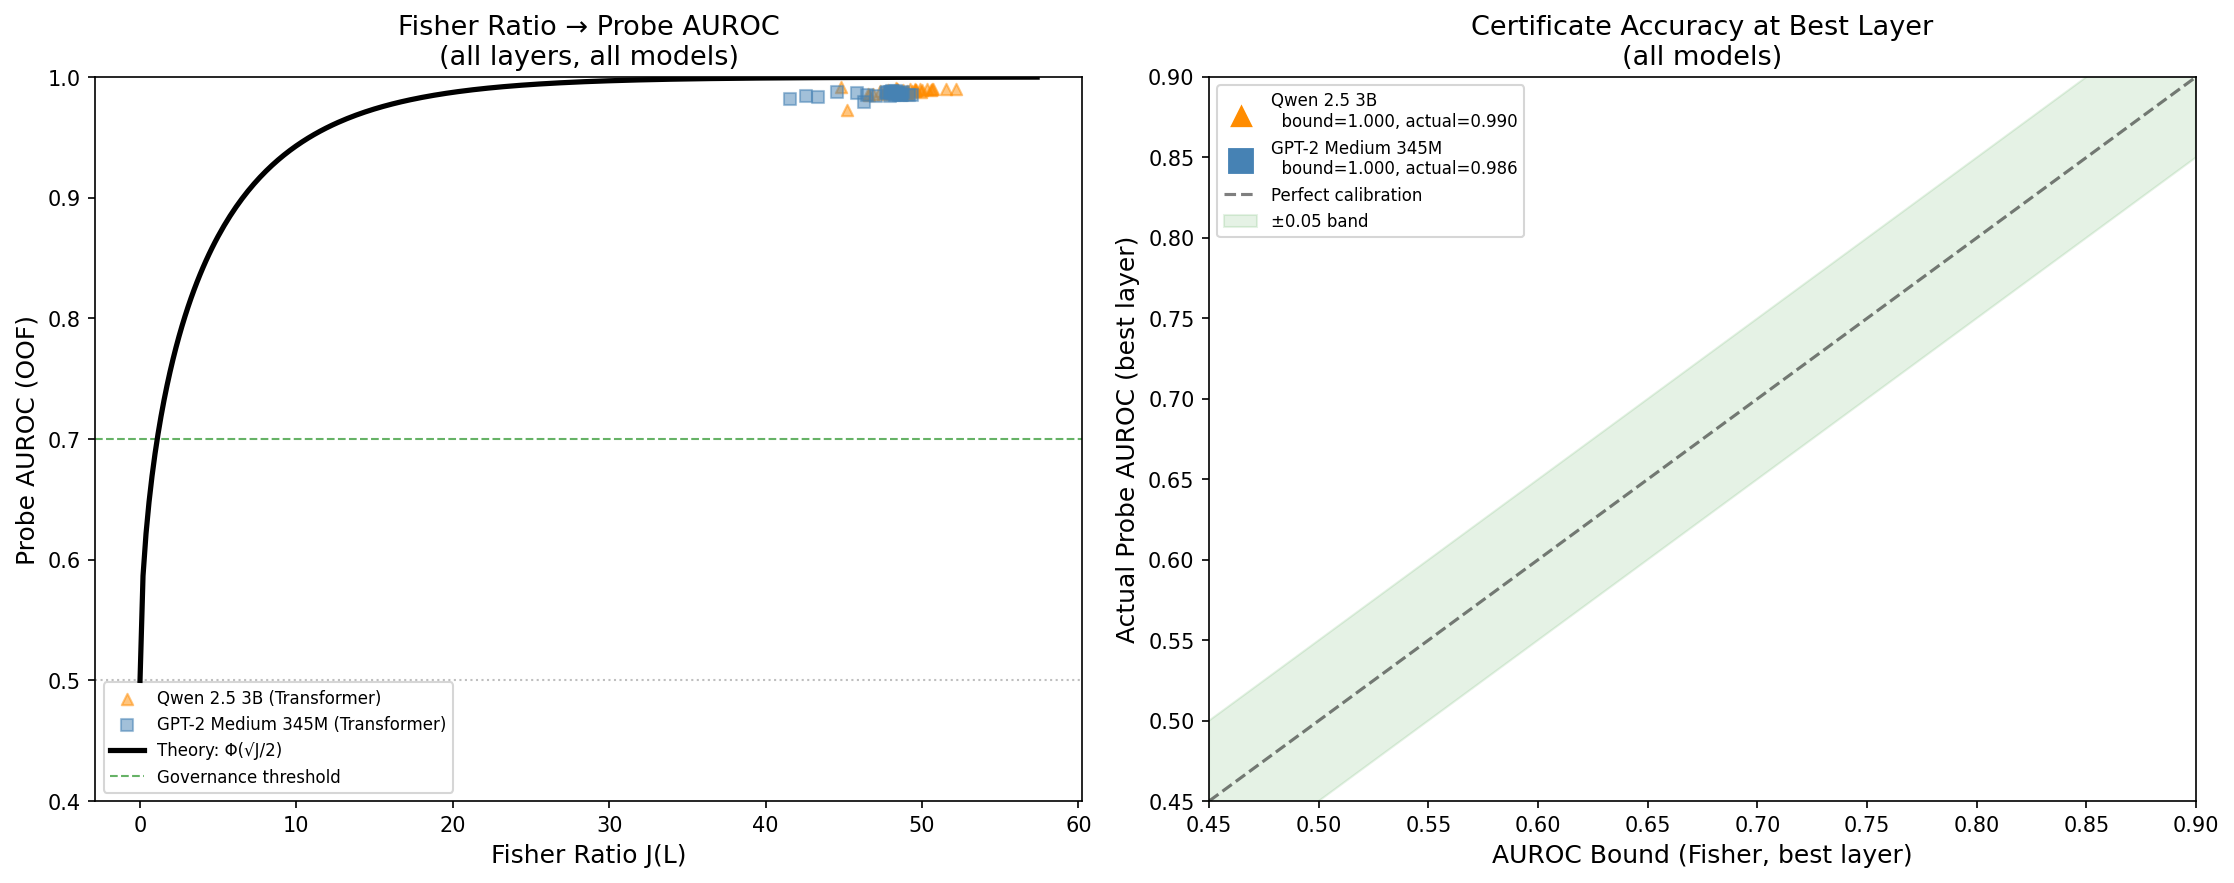
\includegraphics[width=\linewidth]{figures/06_central_figure.png}
\caption{Actual probe AUROC (x-axis) vs.\ Fisher bound $\Phi(\sqrt{J/2})$
  (y-axis) at every layer for Qwen~2.5~3B (blue) and GPT-2~Medium (orange).
  All points lie above the identity line ($\text{bound} \geq \text{actual}$),
  confirming the approximation as a valid upper bound.
  Vertical spread reflects Gaussian assumption violation at high-AUROC layers.}
\label{fig:central}
\end{figure}

\subsection{5-Fold Cross-Validation of the Certificate}
\label{sec:cert-cv}

To simulate the deployment scenario -- predicting probe AUROC on
unseen data -- we run 5-fold CV on Qwen~2.5~3B (Exp.~03). On each
training fold, we compute $J(L)$ and predict the bound. On the held-out
test fold, we measure actual probe AUROC. Table~\ref{tab:cv} reports
fold-level results.

\begin{table}[!htbp]
\centering
\caption{5-fold cross-validation of the certificate (Qwen~2.5~3B,
  $n=2000$, Exp.~03).}
\label{tab:cv}
\small
\setlength{\tabcolsep}{4pt}
\resizebox{\columnwidth}{!}{%
\begin{tabular}{cccccc}
\toprule
\textbf{Fold} & \textbf{Pred.\ Layer} & \textbf{Bound} &
  \textbf{Actual AUROC} & \textbf{Error} & \textbf{Match?} \\
\midrule
1 & L25 & 0.9999 & 0.9845 & 0.0154 & \texttimes \\
2 & L25 & 0.9999 & 0.9847 & 0.0152 & \texttimes \\
3 & L25 & 0.9998 & 0.9930 & 0.0069 & \texttimes \\
4 & L26 & 0.9999 & 0.9935 & 0.0063 & \texttimes \\
5 & L25 & 0.9998 & 0.9974 & 0.0024 & \texttimes \\
\midrule
\multicolumn{2}{l}{Mean} & & & 0.0093 & 0/5 \\
\multicolumn{2}{l}{Std}  & & & 0.0052 & \\
\bottomrule
\end{tabular}}
\end{table}

Mean bound error is $0.93\%$, confirming the certificate's predictive
utility (Figure~\ref{fig:calibration}). However, the predicted layer
(argmax $J$) never matches the oracle best probe layer, across all five
folds (0\% layer-match rate) -- a systematic failure we discuss in
Section~\ref{sec:cert-layer}.

\begin{figure}[h]
\centering
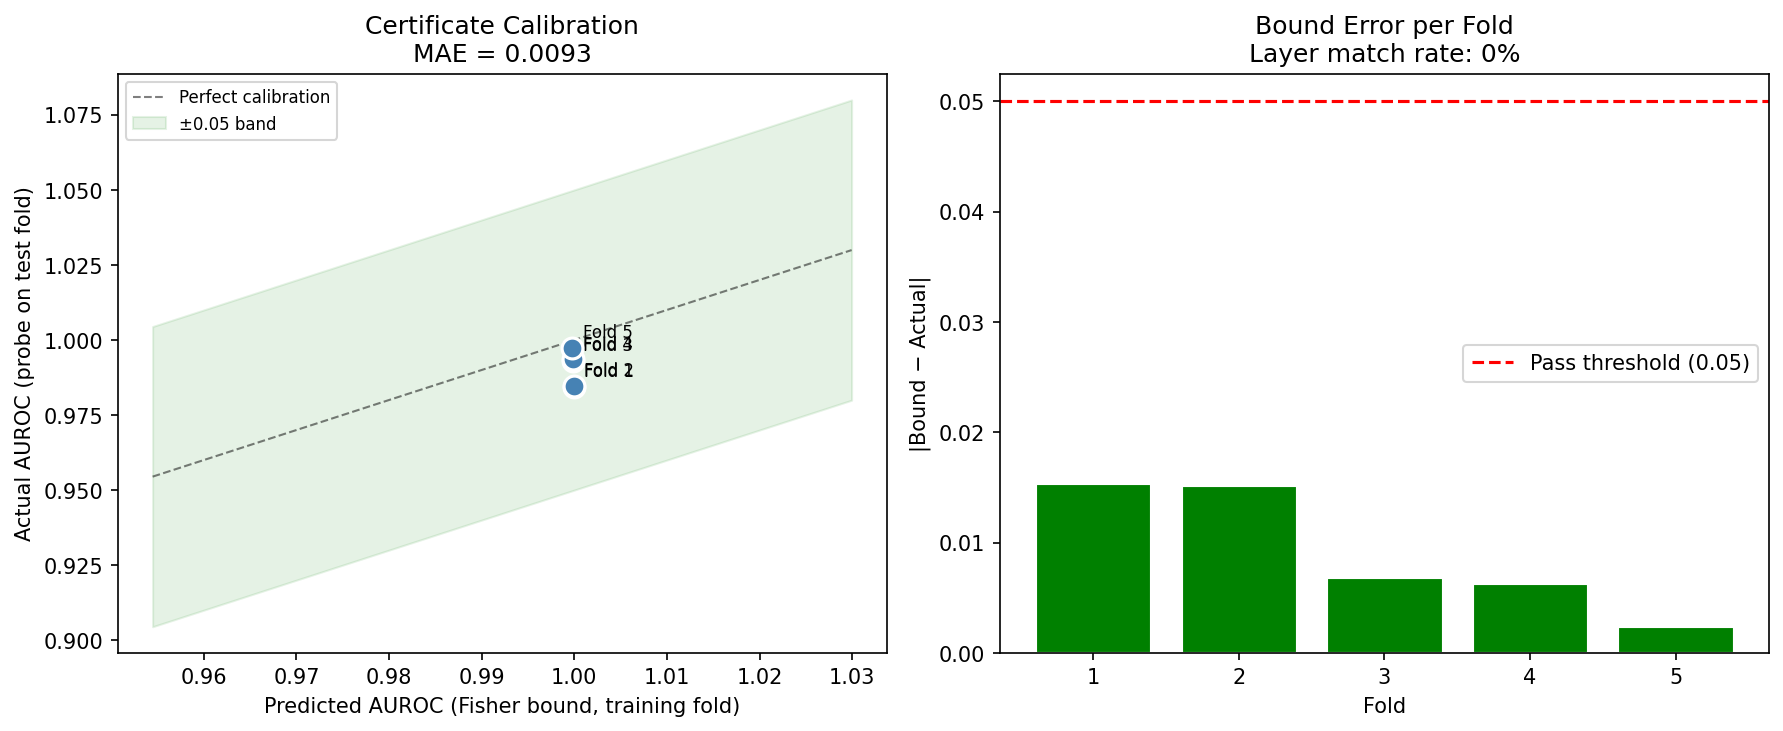
\includegraphics[width=\linewidth]{figures/03_certificate_calibration.png}
\caption{Certificate calibration: predicted bound vs.\ actual AUROC across
  5 cross-validation folds (Qwen~2.5~3B).  The bound consistently
  over-predicts AUROC by $0.6$--$1.5\%$, reflecting systematic Gaussian
  over-estimation.}
\label{fig:calibration}
\end{figure}

\subsection{The Layer Selection Problem}
\label{sec:cert-layer}

Fisher $J$ cannot identify the optimal probing layer. In all five CV
folds, argmax$_L\, J(L)$ selects L25--L26, while oracle best probe
layers range from L10 to L36 across folds. A depth-weighted heuristic
($J(L) \times L / L_{\max}$) achieves a 20\% match rate -- better than
argmax, but still poor.

\begin{remark}
The failure arises because $J$ measures second-order geometry: class
separation by covariance-weighted distance. Probe AUROC instead reflects
the total discriminative structure, including local density variations
and higher-order moments. High $J$ implies high \emph{achievable} AUROC.
It does not identify which layer's probe will realise that potential.
\end{remark}

This is a fundamental limitation: separability does not imply
accessibility by simple probes. The practical implication: the
certificate is useful for deciding \emph{whether} to probe, not
\emph{where}.

\subsection{Competing Geometric Certificates}
\label{sec:cert-competing}

To assess Fisher $J$ relative to alternative geometry-based
certificates, Exp.~01 also evaluates two competitors on the same
hidden-state extractions. \textbf{Local Intrinsic Dimensionality} (LID)
measures the local manifold dimension around each sample.
\textbf{Causal Fisher} first projects hidden states through the causal
residual-stream path, before computing $J$. Table~\ref{tab:competing}
summarises the results.

\begin{table}[!htbp]
\centering
\caption{Competing geometric certificates (Exp.~01). LID peaks at the
  embedding layer (L0) for both models, indicating that intrinsic
  dimensionality does not locate separability structure.
  Causal Fisher reduces $J$ by $25\%$ on Qwen and fails entirely on
  GPT-2~Medium.}
\label{tab:competing}
\small
\setlength{\tabcolsep}{3pt}
\resizebox{\columnwidth}{!}{%
\begin{tabular}{llccc}
\toprule
\textbf{Model} & \textbf{Certificate} & \textbf{Peak Layer} &
  \textbf{Value} & \textbf{Notes} \\
\midrule
\multirow{3}{*}{Qwen 2.5 3B}
  & Fisher $J$ (Euclidean) & L25 & $J = 52.15$ & reference \\
  & Causal Fisher          & L25 & $J = 39.13$ & $-25\%$ vs.\ Euclidean \\
  & LID                    & L0  & AUROC $= 0.949$ & embedding layer \\
\midrule
\multirow{3}{*}{GPT-2 Medium}
  & Fisher $J$ (Euclidean) & L19 & $J = 49.33$ & reference \\
  & Causal Fisher          & ---  & \textit{failed} & projection collapses \\
  & LID                    & L0  & AUROC $= 0.959$ & embedding layer \\
\bottomrule
\end{tabular}}
\end{table}

Three findings follow.
\textit{First}, LID peaks at layer~0 for both models. The embedding
layer carries high intrinsic dimensionality, but this reflects
vocabulary-space geometry, not hallucination class structure: LID AUROC
at L0 is $0.949$ (Qwen) and $0.959$ (GPT-2), driven by surface-form
statistics rather than separability. As a certificate, LID points to the
wrong layer.
\textit{Second}, Causal Fisher reduces $J$ from $52.15$ to $39.13$ on
Qwen~2.5~3B. The causal projection removes correlated non-causal
dimensions that nonetheless carry discriminative information. The
certificate becomes stricter but less tight.
\textit{Third}, Causal Fisher fails entirely on GPT-2~Medium. There, the
smaller residual-stream dimensionality collapses the causal projection
to a near-degenerate subspace.

These comparisons establish Euclidean Fisher $J$ as the strongest of
the three geometry-based certificates. This motivates its central role
in the analysis that follows.

\subsection{Certificate Generalisation to Nonlinear Probes}
\label{sec:mlp-probe}

The Gaussian AUROC bound $\Phi(\sqrt{J/2})$ is derived for linear
classifiers under equal-covariance Gaussian assumptions. A natural
question is whether it also constrains \emph{nonlinear} probes, which
can exploit higher-order representational structure beyond
second-moment geometry.

We address this directly via Exp.~12. We train a shallow MLP probe (64
hidden units, ReLU, Adam, early stopping) on the same PCA(100)-projected
hidden states, using the identical 5-fold stratified CV as the linear
probe. Table~\ref{tab:mlp} reports results.

\begin{table}[!htbp]
\centering
\caption{Fisher certificate vs.\ linear and MLP probes (Exp.~12, 13,
  $n=2000$, 5-fold OOF).  The Fisher bound $\Phi(\sqrt{J/2})$ is never
  violated across all layer--model combinations.
  Qwen~7B row from Exp.~13 (same pipeline, same preprocessing).
  Linear AUROC values may differ slightly across experiments due to
  stochastic 5-fold CV fold assignment.}
\label{tab:mlp}
\small
\setlength{\tabcolsep}{3pt}
\resizebox{\columnwidth}{!}{%
\begin{tabular}{lccccc}
\toprule
\textbf{Model} & \textbf{Bound} & \textbf{Linear} & \textbf{MLP} &
  \textbf{Gain} & \textbf{Viol.} \\
\midrule
Qwen 2.5 3B  & 0.9998 & 0.9903 (L22) & 0.9912 (L20) & $+0.0009$ & 0 / 37 \\
GPT-2 Medium & 0.9998 & 0.9859 (L8)  & 0.9867 (L19) & $+0.0007$ & 0 / 25 \\
Qwen 2.5 7B  & $\approx$1.000 & 0.9998 (L24) & 0.9998 (L9) & $<$0.0001 & 0 / 29 \\
\midrule
\multicolumn{6}{l}{\textit{Mean bound gap (linear):} 0.013 (Qwen 3B),\; 0.017 (GPT-2),\; 0.0005 (Qwen 7B)} \\
\multicolumn{6}{l}{\textit{Mean bound gap (MLP):}    0.013 (Qwen 3B),\; 0.017 (GPT-2),\; 0.0009 (Qwen 7B)} \\
\bottomrule
\end{tabular}}
\end{table}

\begin{figure}[h]
\centering
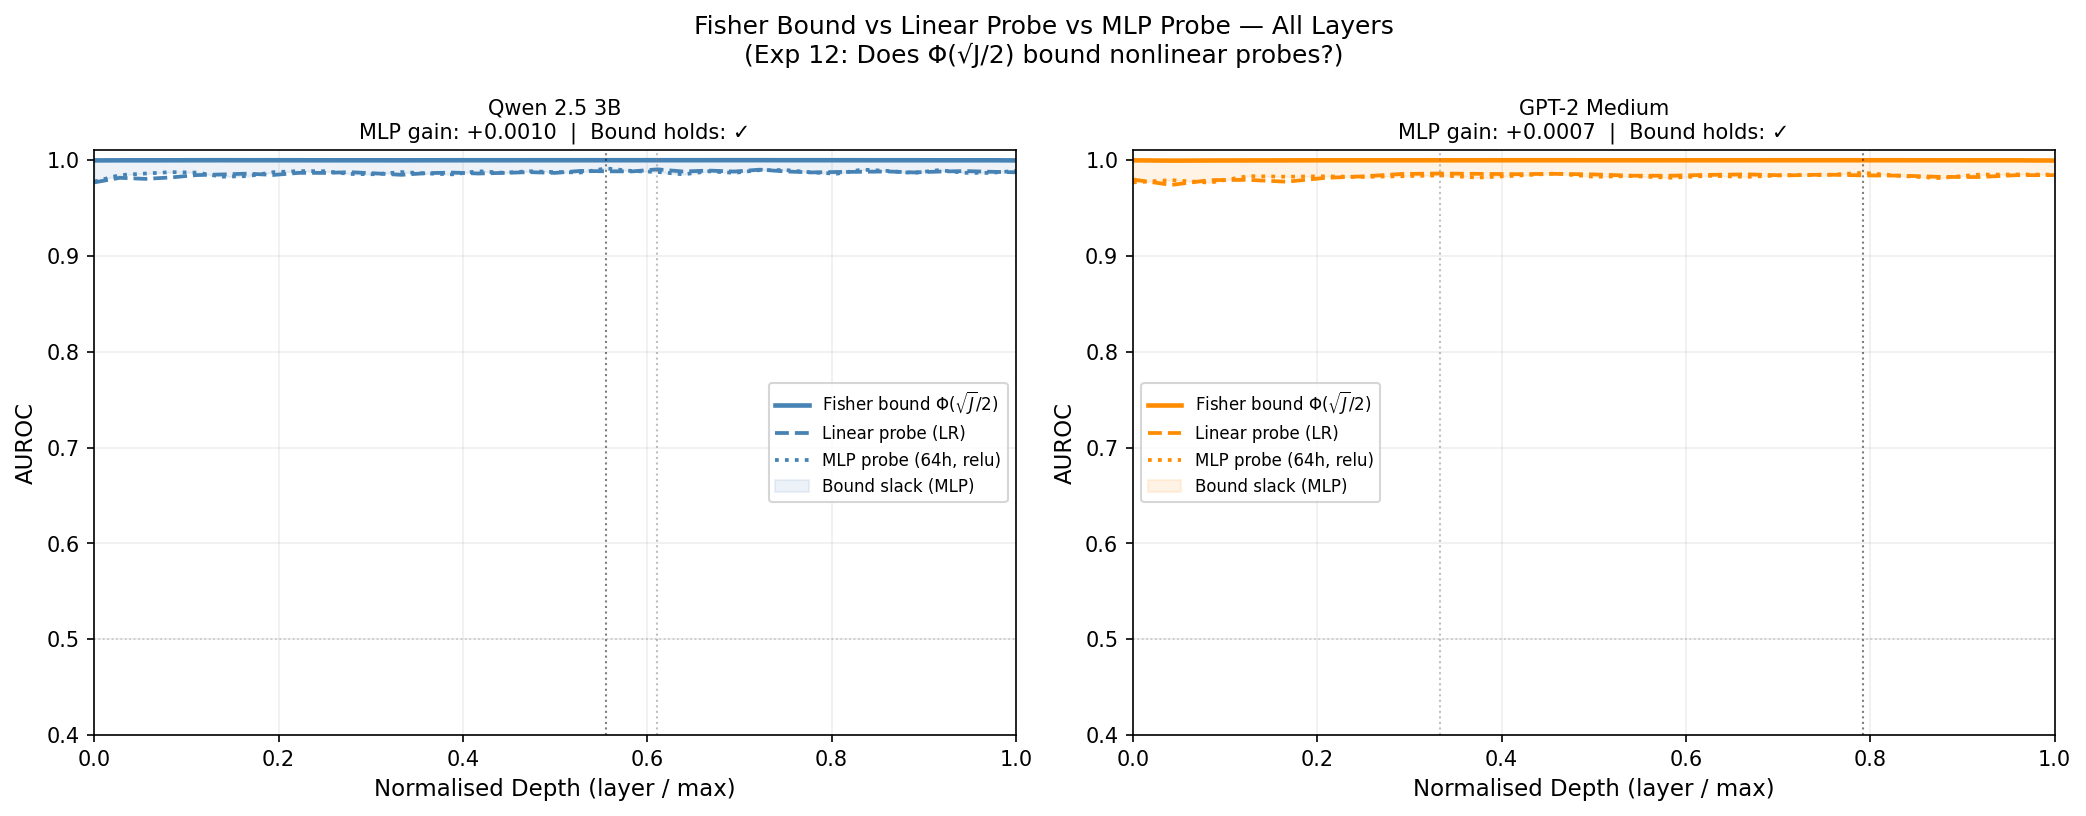
\includegraphics[width=\linewidth]{figures/12_mlp_probe_comparison.png}
\caption{Fisher bound $\Phi(\sqrt{J/2})$ (solid), linear probe AUROC
  (dashed), and MLP probe AUROC (dotted) at every layer.  The shaded
  region is the bound slack.  The bound is never violated by the MLP probe
  on either model.}
\label{fig:mlp}
\end{figure}

Four findings emerge (Figure~\ref{fig:mlp}).
\textit{First}, the MLP probe outperforms the linear probe at $21/37$
layers (Qwen) and $10/25$ layers (GPT-2). This confirms that some
nonlinear structure exists in the representations. The margin is small:
$+0.09\%$ and $+0.07\%$ at best layer respectively.
\textit{Second}, the Fisher bound $\Phi(\sqrt{J/2})$ holds across all
$37 + 25 + 29 = 91$ layer--model combinations, including Qwen~2.5~7B
(zero violations). The Gaussian slack is sufficient to absorb the
additional nonlinear capacity across all tested scales.
\textit{Third}, the mean bound gap narrows only marginally for MLP
vs.\ linear ($0.0133 \to 0.0129$ on Qwen; essentially unchanged on
GPT-2). The MLP does not approach the Gaussian ceiling any more closely
than the linear probe does.
\textit{Fourth}, the MLP and linear probes identify different optimal
layers (Qwen: L20 vs.\ L22; GPT-2: L19 vs.\ L8). This compounds the
layer-selection failure of Section~\ref{sec:cert-layer}.

\textbf{Why the MLP does not beat the certificate.}
The Gaussian derivation of $\Phi(\sqrt{J/2})$ bounds the Bayes-optimal
linear classifier under equal-covariance assumptions. That the MLP also
stays below the same ceiling is informative. It means the
representations themselves, not the probe's functional form, are the
binding constraint. The MLP can only exploit what the hidden-state
geometry provides; it cannot manufacture discriminative structure that
is not already present. The small gain ($\leq 0.09\%$) indicates that
most of the available geometric signal is already captured by
second-moment statistics -- higher-order structure exists, but is
marginal. This is the core finding: \emph{detection performance is a
property of the representation, not of the classifier}.

\begin{remark}[Scope of the nonlinear bound]
The observation that $\Phi(\sqrt{J/2})$ also upper-bounds MLP probe
AUROC is \textbf{empirical, not theoretical}. The Gaussian derivation of
Proposition~\ref{prop:cert} is strictly valid only for linear
classifiers under equal-covariance Gaussian assumptions. It provides no
theoretical guarantee for nonlinear probes. The zero-violation result
across 91 pairs means that, on these specific representations with this
specific shallow architecture, the Gaussian slack happened to absorb
the additional nonlinear capacity. A different architecture (deeper
MLP, kernel methods, attention), or a different dataset, may produce
violations. A principled nonlinear certificate -- one that
characterises higher-order moment structure -- remains an open
theoretical problem.
\end{remark}

% ══════════════════════════════════════════════════════════════════════════════
\FloatBarrier
\section{Scale Behavior}
\label{sec:scale}

\subsection{Within-Family Scaling}
\label{sec:scale-curve}

\textbf{Correction, added post-review (third round): the table and
sigmoid fit in this subsection are superseded by
Table~\ref{tab:certificate-matched}.} They should not be read as a
scale-vs-AUROC finding in their own right. We retain them only because
the sigmoid-fit provenance issue below -- a 3-point fit vs.\ a 7B
out-of-sample check -- is itself an instructive correction.
Table~\ref{tab:scale} mixes Pipeline~B (0.5B, 1.5B: real generation,
ROUGE-L) with Pipeline~A (3B, 7B: forced-choice, no generation). It
reports probe AUROC \emph{rising} with scale (0.813 $\to$ 0.979 $\to$
0.9917 $\to$ 0.9998). Table~\ref{tab:certificate-matched}, under one
matched real-generation pipeline, reports the same four models' probe
AUROC \emph{falling} with scale (0.584 $\to$ 0.602 $\to$ 0.572 $\to$
0.525). These are not two independent findings in tension. The rising
curve below is the pipeline-confounded one, and should be read as
historical/superseded, not as a competing scale law. We fit a sigmoid
scaling curve within the Qwen~2.5 family, to control for architecture,
tokenizer, and training distribution (Exp.~11, 13). Qwen~2.5~7B is
included via Exp.~13 (balanced HaluEval, $n=2000$), replacing the
extrapolated prediction with an actual measurement. Table~\ref{tab:scale}
and Figure~\ref{fig:scale} report AUROC at best layer for each model
\emph{under the superseded, cross-pipeline methodology}.

\begin{table}[!htbp]
\centering
\caption{Qwen~2.5 family: best-layer probe AUROC vs.\ model scale
  (Exp.~11, 13; $n = 400$ controlled for 0.5B--3B; $n=2000$ for 7B).
  $^\ddagger$7B: Exp.~13 actual measurement, replacing the extrapolated
  prediction from Exp.~11.}
\label{tab:scale}
\small
\setlength{\tabcolsep}{5pt}
\resizebox{\columnwidth}{!}{%
\begin{tabular}{lrrrr}
\toprule
\textbf{Model} & \textbf{Params} & \textbf{Best AUROC} &
  \textbf{Best Layer} & \textbf{Depth} \\
\midrule
Qwen 2.5 0.5B & 494M  & 0.813  & L7  & 29\% \\
Qwen 2.5 1.5B & 1.54B & 0.979  & L15 & 54\% \\
Qwen 2.5 3B   & 3.09B & 0.9917 & L36 & 100\%\\
Qwen 2.5 7B$^\ddagger$ & 7.6B & 0.9998 & L24 & 86\% \\
\midrule
\multicolumn{5}{l}{\textit{3-point sigmoid fit (0.5B/1.5B/3B only): }
  $\hat{\sigma}(4.71 \cdot \log_{10}(P) - 39.45)$,\;\; $R^2 = 0.9996$} \\
\bottomrule
\end{tabular}}
\end{table}

\textbf{Correction, added post-review (second round):} an earlier
draft labeled this a ``4-point sigmoid fit (0.5B--7B)'' and claimed all
four measurements were directly observed inputs to the fit. Checking
\texttt{results/logs/11\_qwen\_scale\_curve.json} directly:
\texttt{controlled\_scale\_fit} (whose coefficients $a=4.707$,
$b=-39.449$, $R^2=0.99956$ match the rounded values quoted above) is
computed from exactly \emph{three} points -- 0.5B, 1.5B, and 3B. Its own
\texttt{caveat\_n\_points} field states ``fit on only 3 data points.''
The 7B point is not part of the fit at all; it is an \emph{out-of-sample
prediction target}. The fitted curve predicts
$\hat{\text{AUROC}}(7.6\text{B}) = 0.99899$, with a bootstrapped 90\% CI
of $[0.99854, 0.99913]$ (\texttt{prediction\_7b}, $5000$ bootstrap
resamples). \textbf{Final-audit clarification:} this CI is stored as a
top-level sibling key in the JSON, rather than nested under
\texttt{controlled\_scale\_fit}. But its point estimate, $0.998978506$,
matches \texttt{controlled\_scale\_fit.pred\_7b\_controlled}
($0.998985736$) to 5 decimal places, and not the uncontrolled
\texttt{scale\_fit}'s implied prediction -- confirming it was computed
from the controlled fit despite the JSON's flat key structure. The
actual measured 7B AUROC (Exp.~13) is $0.99981$, which is \emph{above
the upper end of this interval}. The prediction is close in absolute
terms ($0.00083$ gap, still $<0.001$), but is not, strictly, a
successful interval prediction at the stated 90\% confidence level.
$R^2 = 0.9996$ on three points with two free parameters remains far too
few to constitute a scaling law. We report the fit as an
\emph{interpolation} across three measurements, with the 7B point as a
directionally-consistent but interval-missing out-of-sample check, not
a fourth fitted observation.

\begin{figure}[h]
\centering
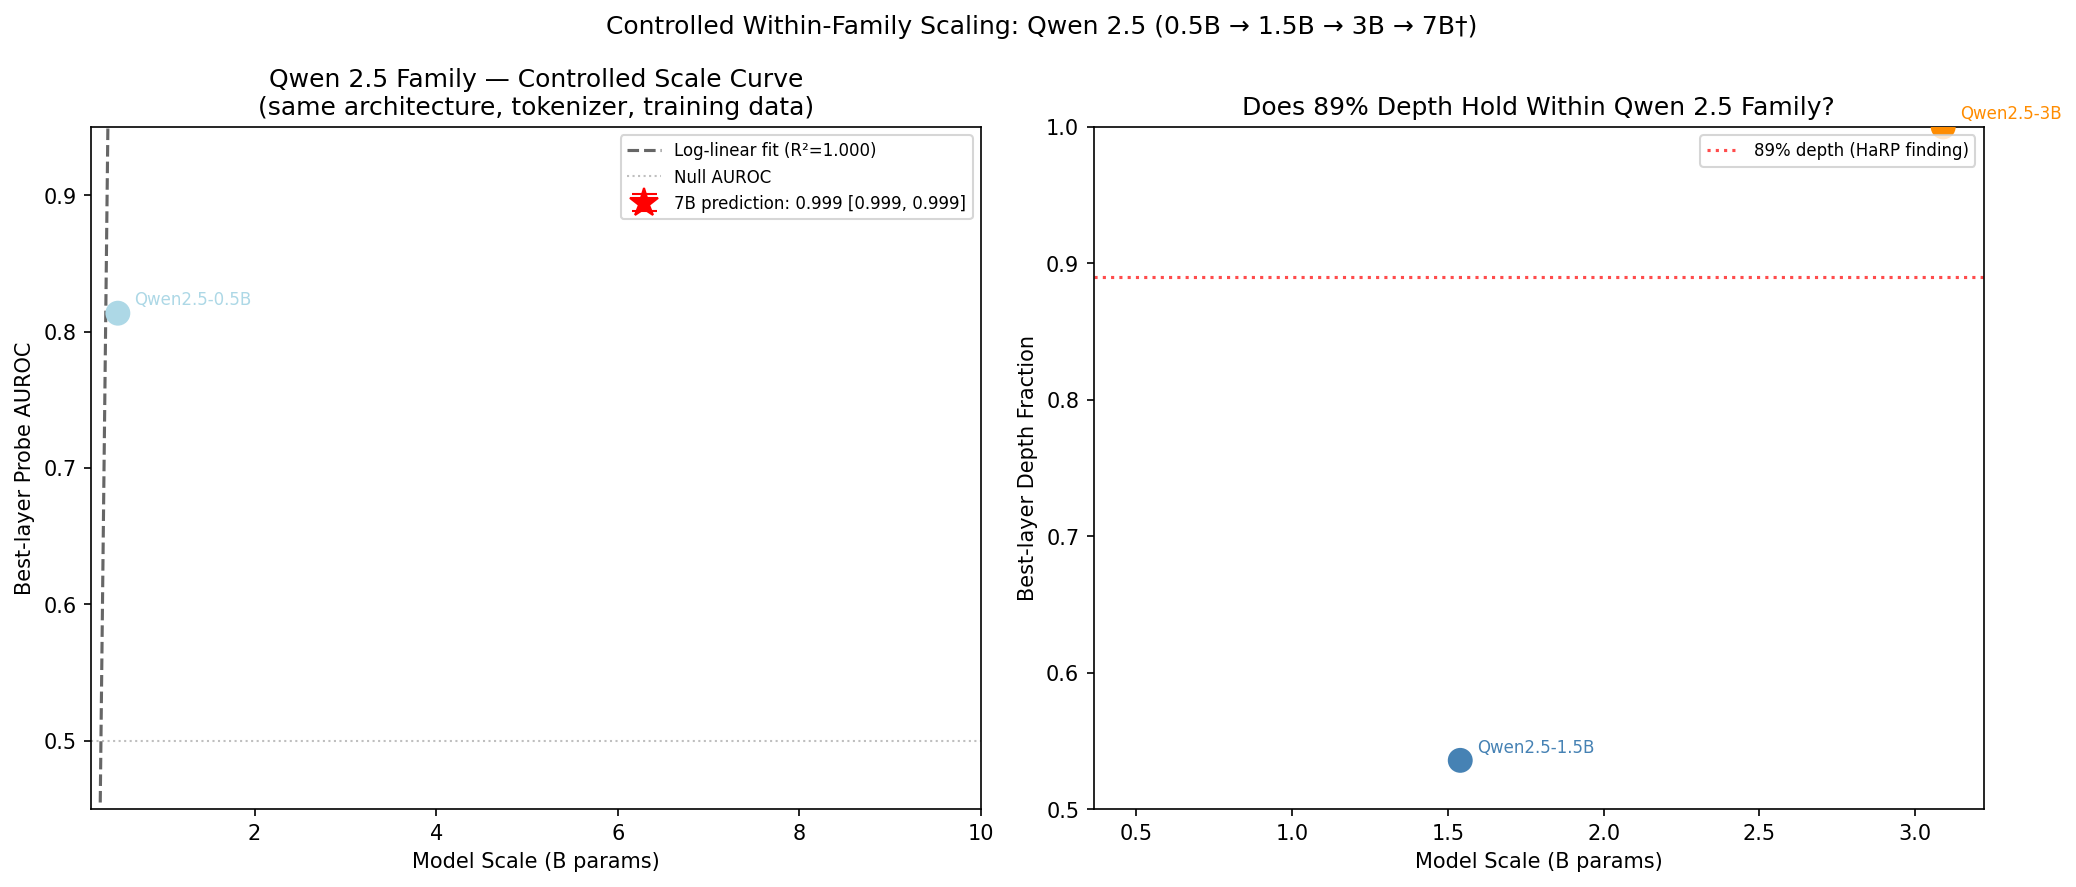
\includegraphics[width=\linewidth]{figures/11_qwen_scale_curve.png}
\caption{\textbf{Superseded by Table~\ref{tab:certificate-matched}
  (see \S\ref{sec:scale-curve}).} Controlled scale curve within the
  Qwen~2.5 family under the cross-pipeline (Pipeline A/B) methodology:
  AUROC appears to grow monotonically with parameter count. The 7B point
  (Exp.~13) replaces the extrapolated prediction with an actual
  measurement. Under the matched Pipeline~C methodology, the same four
  models' AUROC falls with scale instead (Table~\ref{tab:certificate-matched}).}
\label{fig:scale}
\end{figure}

\subsection{Depth Fraction Is Not Universal}
\label{sec:depth}

Table~\ref{tab:depth} compares Fisher-$J$ peak depth and probe-AUROC peak
depth across models (Exp.~05).

\begin{table}[!htbp]
\centering
\caption{Depth fraction of best Fisher-$J$ layer vs.\ best probe-AUROC
  layer (Exp.~05).  Probe peak depth can vary $\pm$2--14 layers across
  independent CV runs; values reflect Exp.~05 fold assignment.}
\label{tab:depth}
\small
\resizebox{\columnwidth}{!}{%
\begin{tabular}{lcc}
\toprule
\textbf{Model} & \textbf{Fisher peak depth} & \textbf{Probe peak depth} \\
\midrule
GPT-2 117M    & 69\% & 69\% \\
GPT-2 Medium  & 79\% & 33\% \\
Qwen 2.5 0.5B & 29\% & 29\% \\
Qwen 2.5 1.5B & 54\% & 54\% \\
Qwen 2.5 3B   & 69\% & 100\%\\
\bottomrule
\end{tabular}}
\end{table}

\begin{figure}[h]
\centering
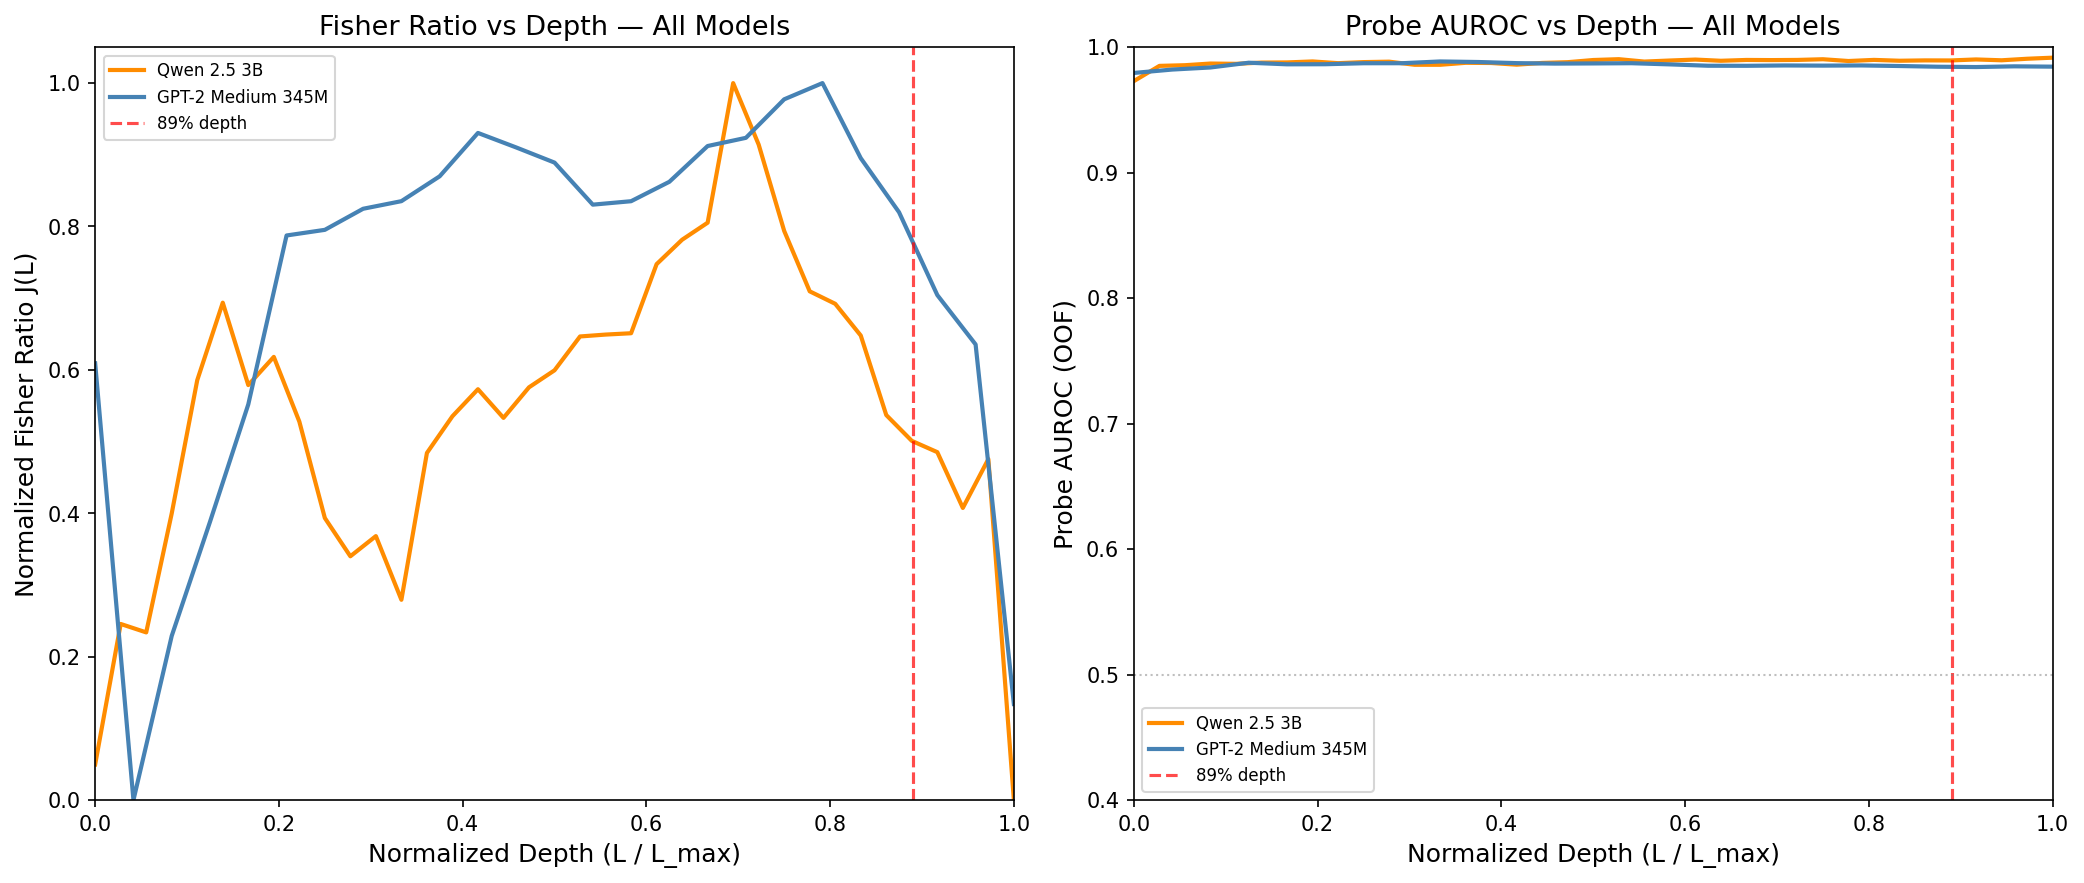
\includegraphics[width=\linewidth]{figures/05_depth_fraction_overlay.png}
\caption{Normalised-depth curves of Fisher $J$ (solid) and probe AUROC
  (dashed) for Qwen~2.5~3B and GPT-2~Medium.  Fisher and probe peaks
  disagree substantially for both models, confirming the layer-selection
  failure of Section~\ref{sec:cert-layer}.}
\label{fig:depth}
\end{figure}

No universal depth fraction emerges (Figure~\ref{fig:depth}). Within
Qwen~2.5, the best layer shifts from $29\%$ (0.5B) to $54\%$ (1.5B) to
$100\%$ (3B). Depth is scale-dependent, not architecture-constant.

An earlier draft reported that Fisher $J$ at best layer is
\emph{non-monotone} with scale within the Qwen family (Qwen 0.5B: $J =
24.5$; Qwen 1.5B: $J = 125.1$; Qwen 3B: $J = 51.8$; Qwen 7B: $J =
184.7$ -- peaking at 1.5B, dropping at 3B, rising again at 7B). It
flagged -- correctly, as far as it went -- that the 1.5B point also had
the worst covariance-estimation reliability in the study (aspect ratio
$\gamma = d/n = 3.84$, \S\ref{sec:setup-fisher}). This left open
whether the non-monotonicity was a genuine geometric property or an
estimation artifact.

\textbf{Two-stage resolution (Exp.~15, then a direct confound check):
the original non-monotonicity was a cross-pipeline task confound. What
looked like its clean replacement -- a monotone trend -- was, in turn, a
minority-class sample-size artifact. Neither the original claim nor its
first replacement survives.} The four points above mixed Pipeline~B
(0.5B, 1.5B: real generation, ROUGE-L, near-degenerate labels) with
Pipeline~A (3B, 7B: forced-choice, no generation). Table~\ref{tab:certificate-matched}
reran all six models under one real-generation, consistently-labeled
pipeline. It initially appeared to find $J$ \emph{perfectly monotone
decreasing} with scale (Spearman $\rho=-1.0$). We directly tested this
by subsampling every model's minority (correct) class to a fixed
$n=24$ (matching the smallest available class, 30 resamples per model,
same Fisher estimator). This makes the monotone trend disappear
($\rho=+0.54$, $p=0.27$, sign reversed from the unmatched analysis) --
see \S\ref{sec:cert-validation}, where we withdraw this claim in full.
The high-$\gamma$ covariance concern for the original 1.5B point was a
reasonable caveat to raise, given the information available at the
time. The underlying intuition -- small-sample covariance/mean
estimation distorting $J$ -- turned out to be exactly correct, just
operating through minority-class size rather than the aspect-ratio
$\gamma$ specifically. The honest resolution of this subsection's
original question is this: once both the cross-pipeline confound
\emph{and} the minority-class-size confound are controlled for, there
is no reliable monotone (or non-monotone) relationship between Fisher
$J$'s magnitude and model scale in this data, in either direction.
Depth \emph{fraction} non-universality -- this subsection's original,
narrower claim -- is untouched by this correction and stands as
originally reported. It is unaffected by either confound, since it
compares relative position within a single model's own layer sweep.

% ══════════════════════════════════════════════════════════════════════════════
\FloatBarrier
\section{Beyond Gaussianity: Wasserstein Certificates}
\label{sec:ot}

\subsection{The Fisher--Wasserstein Identity and Its Violation}
\label{sec:ot-identity}

Under Gaussian equal-covariance assumptions, Fisher separability and
Wasserstein-2 distance in whitened space are identical:
$J = W_2^2\!\left(\tilde{P}_c, \tilde{P}_h\right)$, where $\tilde{P} =
\Sigma_w^{-1/2} P$.
We verify this identity at five representative layers per model
(Exp.~08). Table~\ref{tab:identity} reports relative errors
$\epsilon = |J - W_{2,\text{wh}}^2| / J$.

\begin{table}[!htbp]
\centering
\caption{Relative error of $J \approx W_2^2$ (whitened) identity at
  five layers per model (Exp.~08).  Identity never holds; error grows
  with depth for Qwen.}
\label{tab:identity}
\small
\setlength{\tabcolsep}{4pt}
\resizebox{\columnwidth}{!}{%
\begin{tabular}{lcccccc}
\toprule
\textbf{Model} & \textbf{L0} & \textbf{L$\nicefrac{1}{4}$} &
  \textbf{L$\nicefrac{1}{2}$} & \textbf{L$\nicefrac{3}{4}$} &
  \textbf{L$_{\max}$} & \textbf{Mean} \\
\midrule
Qwen 2.5 3B  & 0.72 & 1.43 & 1.64 & 1.76 & 3.01 & 1.71 \\
GPT-2 Medium & 0.54 & 0.83 & 0.87 & 0.75 & 0.88 & 0.77 \\
\bottomrule
\end{tabular}}
\end{table}

The identity $J = W_2^2$ fails across all layers: mean relative error
$1.71$ for Qwen, $0.77$ for GPT-2. This is a \emph{finding} --
hidden-state distributions are measurably
non-Gaussian~\citep{disipio2025fisher} -- not a flaw in the
experimental design.

\subsection{\texorpdfstring{SW$_2$}{SW2} vs.\ Fisher for AUROC Prediction}
\label{sec:ot-sw2}

We compare four certificates -- Fisher $J$, Sliced Wasserstein
($\text{SW}_2$), Bures $W_2$, and MMD$^2$ -- via Spearman $\rho$ with
probe AUROC across all layers (Exp.~08). Table~\ref{tab:ot} reports results.

\begin{table}[!htbp]
\centering
\caption{Spearman $\rho$ between certificate value and probe AUROC across
  all layers (Exp.~08).  Higher is better.  Bures~$W_2$ and SW$_2$ both
  substantially outperform Fisher on Qwen (best: Bures 0.828, bold);
  Fisher wins on GPT-2.  SW$_2$ and Bures~$W_2$ are distribution-free;
  the 0.007 gap between them is within noise.}
\label{tab:ot}
\small
\setlength{\tabcolsep}{4pt}
\resizebox{\columnwidth}{!}{%
\begin{tabular}{lcccc}
\toprule
\textbf{Model} & \textbf{Fisher~$J$} & \textbf{SW$_2$} &
  \textbf{Bures~$W_2$} & \textbf{MMD$^2$} \\
\midrule
Qwen 2.5 3B  & 0.458 & 0.821 & \textbf{0.828} & 0.542 \\
GPT-2 Medium & \textbf{0.395} & $-0.237$ & $-0.241$ & $-0.596$ \\
\bottomrule
\end{tabular}}
\end{table}

\begin{figure}[h]
\centering
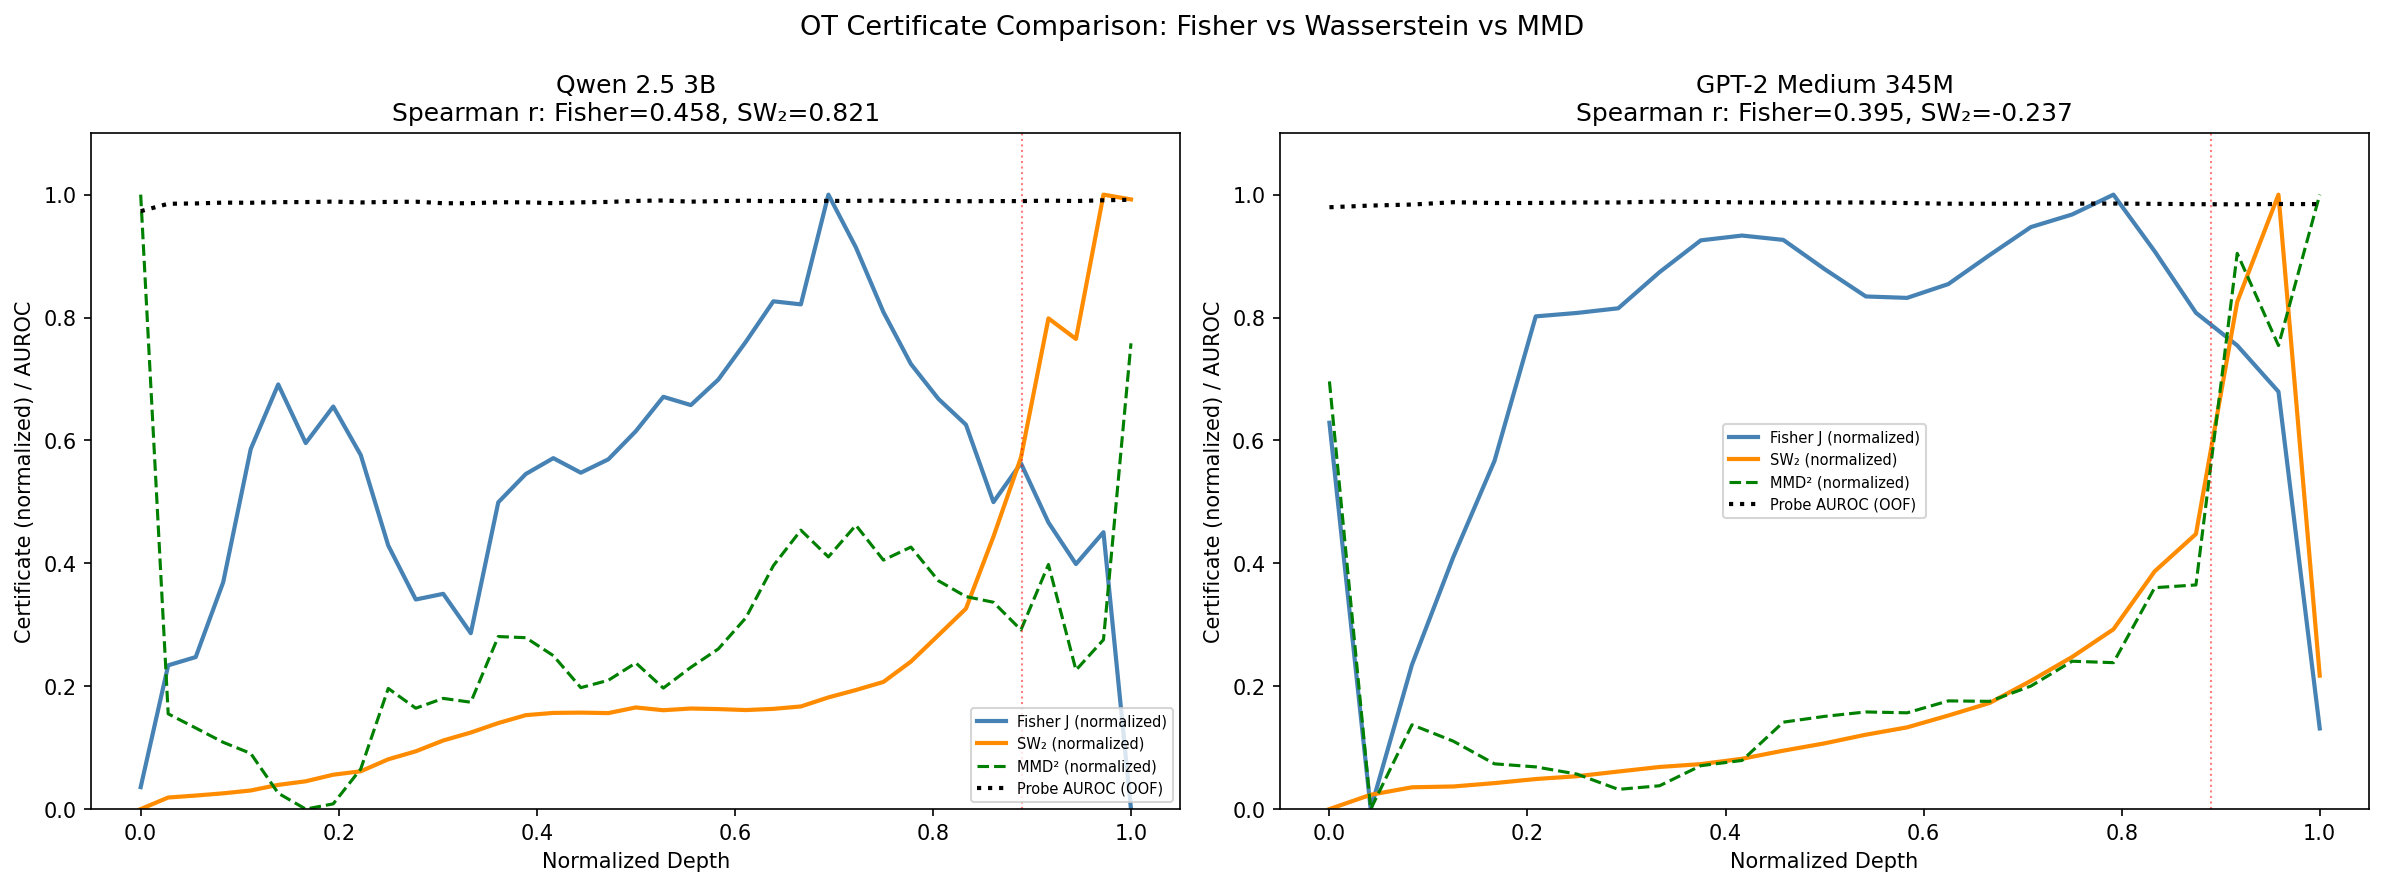
\includegraphics[width=\linewidth]{figures/08_ot_certificates.png}
\caption{Certificate value (normalised) vs.\ layer depth for Qwen~2.5~3B.
  SW$_2$ (orange) grows monotonically and peaks near the probe AUROC peak
  (L36), while Fisher $J$ (blue) is flat across layers.  The flat $J$
  curve explains its low Spearman $\rho$ despite tight bound error.}
\label{fig:ot}
\end{figure}

Both Bures~$W_2$ ($\rho = 0.828$) and SW$_2$ ($\rho = 0.821$)
substantially outperform Fisher on Qwen ($\rho = 0.458$). Bures~$W_2$ is
the marginal leader (by $0.007$, within noise). Both distribution-free
certificates share the same mechanism: monotonic growth across layers
that tracks the probe AUROC trajectory. \emph{This advantage reverses
entirely on GPT-2 Medium} (SW$_2$: $\rho = -0.237$; Bures $W_2$: $\rho =
-0.241$; Fisher: $\rho = 0.395$). There, both distribution-free
certificates grow monotonically in the wrong direction relative to
probe AUROC, which peaks at L8, the earliest layer.
\textbf{Correction, added post-review (second round):} an earlier draft
called this model-dependence of optimal certificate choice ``the
central finding of this section and, we argue, of the paper as a
whole,'' in the same breath as caveating it as an $n=2$ observation --
an internal contradiction; a finding cannot be both. It is neither.
With only two architectures, no bootstrap CI, and a probe-AUROC target
with ${\approx}1$--$2\%$ dynamic range across layers (Table~\ref{tab:ot}:
Qwen 3B ranges $0.973$--$0.992$), this is a \emph{suggestive
two-architecture observation}. It motivates the mechanistic hypothesis
below; it is not a validated claim that no universally superior
distribution-free certificate exists. \textbf{We flag explicitly that
this is an $n=2$ architecture comparison} (Qwen~2.5~3B vs.\ GPT-2
Medium) -- two points establish a reversal, not a law. A third,
architecturally distinct model (e.g.\ Llama or Pythia -- our attempted
Mamba/SSM transfer failed for unrelated reasons,
\S\ref{sec:limitations}), and a fold-level bootstrap CI on each $\rho$,
are needed before ``no universal certificate'' should be read as more
than that.

\begin{remark}[Mechanistic interpretation]
The reversal reflects a difference in representational compression
dynamics. In Qwen~2.5~3B, deeper layers progressively compress hidden
states toward well-separated class manifolds. Distributional divergence
(SW$_2$, Bures $W_2$) grows monotonically with this compression, making
it a natural proxy for linear separability. In GPT-2~Medium, the
optimal probe layer sits at only $33\%$ depth (L8) -- before any
late-layer compression occurs. As depth increases beyond L8,
representational structure becomes \emph{less} discriminative for
hallucination detection, so distributional divergence and probe AUROC
evolve in opposite directions. The implication is architectural: the
certificate choice (Fisher vs.\ distribution-free) is governed by
\emph{when} discriminative structure peaks within the network. This is
itself a function of training objective and architecture, not
parameter count.
\end{remark}

% ══════════════════════════════════════════════════════════════════════════════
\FloatBarrier
\section{Conformal Coverage Guarantees}
\label{sec:conformal}

\subsection{Calibration and Results}
\label{sec:conformal-results}

We apply split conformal prediction on the probe's hallucination score,
at the best probe layer identified in Exp.~10 (L36 for Qwen, L8 for
GPT-2~Medium). The best probe layer varies by $\pm$2--14 layers across
experiments, due to stochastic CV fold assignment. The conformal
guarantee is independent of which specific layer is used: it holds at
any fixed, pre-specified layer. The dataset is split $60/20/20$
(train/calibration/test). We seek the smallest $\alpha^*$ such that
$P(\text{hall} \mid \text{accepted}) \leq \alpha^*$ holds empirically at
coverage $1 - \delta = 0.95$ (Exp.~10).

\begin{table}[!htbp]
\centering
\caption{Conformal guarantee results (Exp.~10, 13, in-distribution).
  Qwen~7B from Exp.~13 (same 60/20/20 split, same calibration protocol).
  $^\S$``$\alpha = 0.10$ holds?'' asks whether the guarantee can be
  satisfied with $> 50\%$ acceptance at the nominal $0.10$ level. All
  models show \texttimes: the high ROUGE-L hallucination rate
  (${\approx}99\%$ globally) causes the hall rate to exceed $0.10$ once
  more than ${\approx}53\%$ of queries are accepted. The tighter
  $\alpha^*$ values are required to achieve formal coverage.}
\label{tab:conformal}
\small
\setlength{\tabcolsep}{4pt}
\resizebox{\columnwidth}{!}{%
\begin{tabular}{lcccc}
\toprule
\textbf{Model} & \textbf{$\alpha^*$} & \textbf{Emp.\ hall rate}
  & \textbf{Accept rate} & \textbf{$\alpha = 0.10$ holds?$^\S$} \\
\midrule
Qwen 2.5 3B  & 0.070 & 0.0605 & 52.9\% & \texttimes \\
GPT-2 Medium & 0.060 & 0.0587 & 52.8\% & \texttimes \\
Qwen 2.5 7B  & 0.040 & 0.0379 & 52.8\% & \texttimes \\
\bottomrule
\end{tabular}}
\end{table}

\begin{figure}[h]
\centering
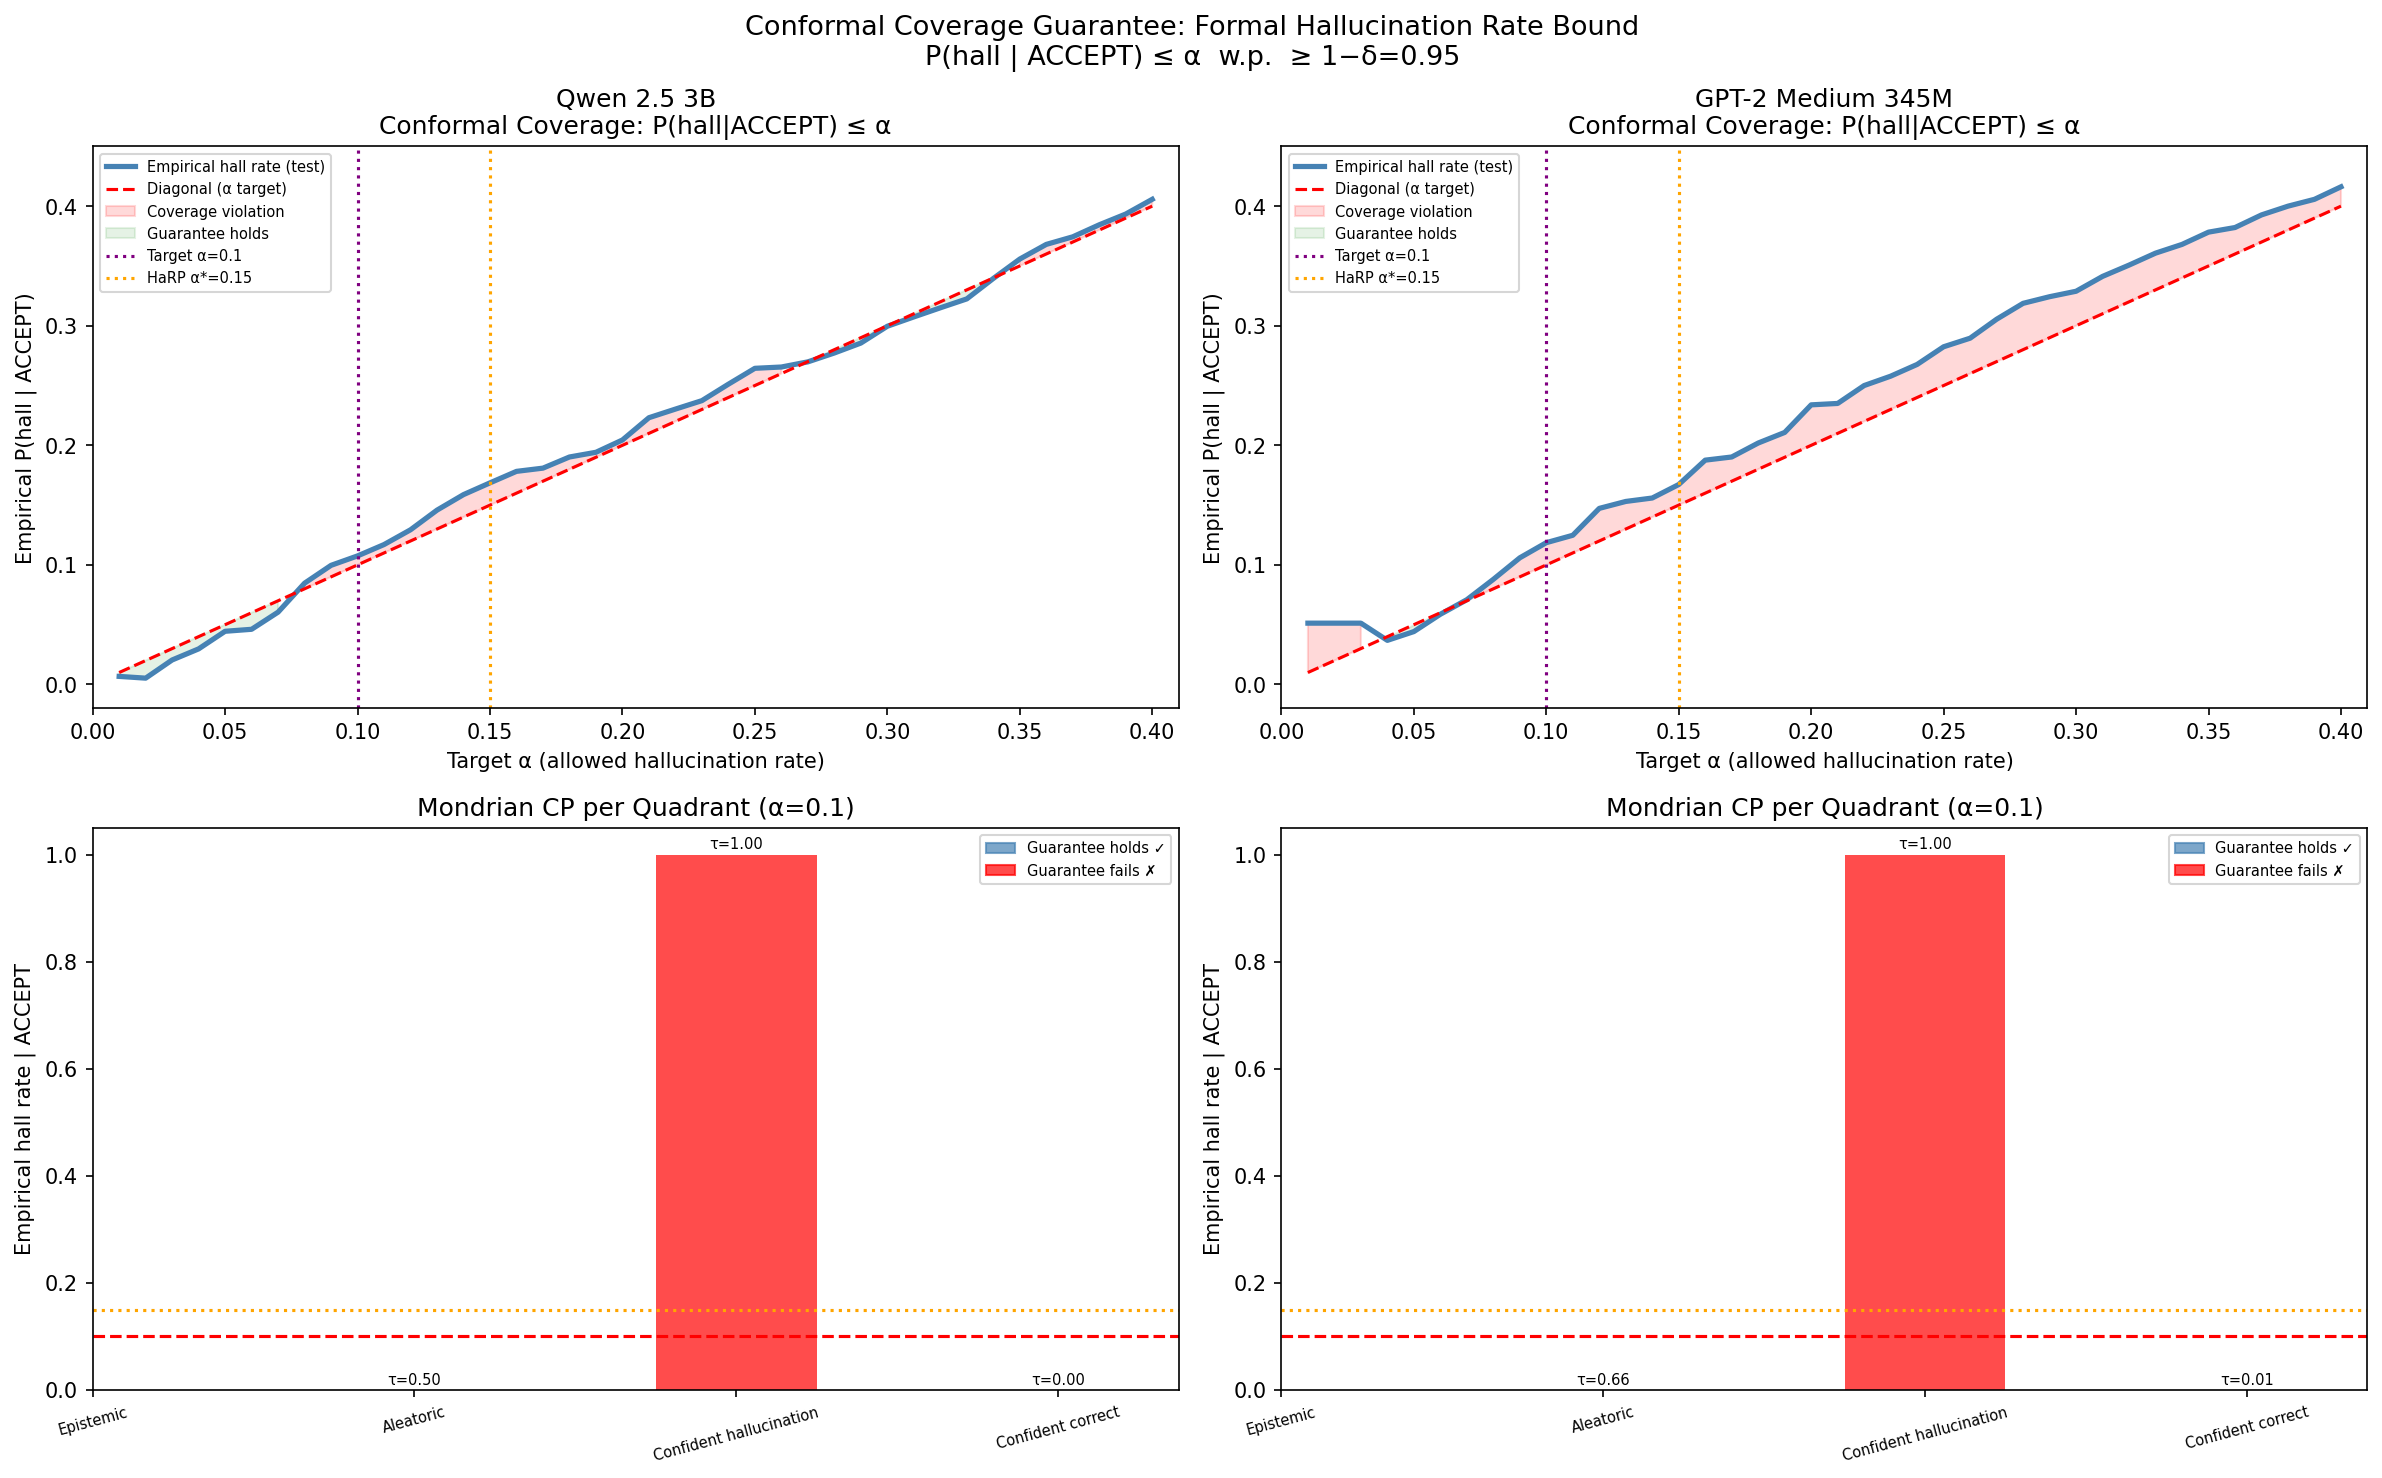
\includegraphics[width=\linewidth]{figures/10_conformal_coverage.png}
\caption{Conformal coverage curve: empirical hallucination rate among
  accepted queries as a function of nominal $\alpha$ (Qwen~2.5~3B).
  The vertical dashed line marks $\alpha^* = 0.07$.  Accepting more
  queries (higher $\alpha$) relaxes the guarantee monotonically.}
\label{fig:conformal}
\end{figure}

At $\alpha^* = 0.07$, the system must reject $47.1\%$ of queries to
achieve the coverage guarantee (Figure~\ref{fig:conformal}).  This
acceptance-rate cost is the honest price of formal coverage.

\subsection{Distribution Shift: Guarantee Collapse}
\label{sec:conformal-ood}

We test conformal thresholds calibrated on HaluEval on 400 TruthfulQA
questions -- a genuinely different task distribution. Both OOD
experiments use a 75/25 train/calibration split on HaluEval, independent
of the 60/20/20 split used in Table~\ref{tab:conformal}. This yields
slightly different $\alpha^*$ values. The violation factor is reported
against the threshold calibrated in each OOD experiment.

\textbf{Correction (post-review):} an earlier draft of this section
attributed the first result below to GPT-2 Medium. Tracing the exact
value back through \texttt{results/logs/10\_conformal\_coverage.json}
shows it is in fact Qwen~2.5~3B's \texttt{real\_ood\_truthfulqa} result.
No real-OOD experiment (as opposed to the simulated-shift check) was
ever run for GPT-2 Medium. We correct the attribution below, and draw
the correspondingly weaker conclusion.

For Qwen~2.5~3B (Exp.~10, real TruthfulQA transfer, $n=400$): AUROC
$= 0.485$; empirical hallucination rate $= 0.982$ (only 7/400 responses
scored correct); a ${\approx}14.0\times$ violation at $\alpha^* = 0.07$.

For Qwen~2.5~7B (Exp.~14): in-distribution AUROC $= 0.9998$ at $L_{24}$
collapses to AUROC $= 0.384$ on TruthfulQA -- \emph{below} chance level.
Acceptance rate $= 100\%$ (threshold accepts everything); empirical
hallucination rate $= 0.993$; violation factor $= 14.2\times$ at
$\alpha^* = 0.07$ (75/25 calibration). The AUROC drop is $0.616$ -- the
most severe collapse observed across all experiments.

\textbf{Correction, added post-review (second round): the near-identical
violation factors are substantially an arithmetic artifact, and this
comparison also inherits the in-distribution/OOD task confound described
in \S\ref{sec:setup-task}.} The violation factor is computed as
(empirical hallucination rate among accepted queries)~$/~\alpha^*$. Both
models' TruthfulQA hallucination rate is pinned to ${\approx}0.98$--$0.99$
by the same underlying cause: TruthfulQA responses are scored via
Pipeline~B (real generation, ROUGE-L~$\geq 0.4$), which registers only
$7/400$ (Qwen~3B) and $3/400$ (Qwen~7B) responses as correct. Both are
near-degenerate label sets, not a meaningfully measured hallucination
rate. Dividing two numbers that are both ${\approx}0.98$--$0.99$ by two
similar $\alpha^*$ values -- both calibrated near $0.07$ on the
\emph{in-distribution, Pipeline-A} HaluEval data -- mechanically
produces similar quotients ($14.0\times$, $14.2\times$), regardless of
whether the underlying collapse mechanism is actually scale-invariant.
Likewise, the reported AUROCs of $0.485$ and $0.384$ are computed
against $7$ and $3$ positive examples respectively out of $400$ -- too
few for AUROC to be a stable or well-defined quantity (a single
relabeled example can move it by several points).
\texttt{results/logs/10\_conformal\_coverage.json} itself notes ``AUROC
undefined if single-class.'' Combined with the Pipeline-A-vs-Pipeline-B
task confound -- in-distribution numbers come from an easier
forced-choice task, OOD numbers come from harder real generation -- the
safest reading of this section is: \emph{both models fail to produce
TruthfulQA answers that clear the ROUGE-L bar, and the conformal
guarantee, calibrated on an easier, different task, provides no usable
coverage once the model is asked to generate freely on a new
distribution.} This is weaker than, but consistent with, the paper's
original framing: \emph{distribution mismatch defeats the guarantee}. It
does \emph{not} license the stronger claim that the collapse mechanism
is quantitatively scale-invariant, since the two violation factors were
never free to differ much, given how both were computed. A genuine test
of scale-invariance would need OOD hallucination rates with enough
positive examples for AUROC to be well-defined, and a labeling pipeline
matched between the in-distribution and OOD arms -- neither holds here.
We retain the qualitative point -- both models' guarantees void
out-of-distribution -- but withdraw the quantitative
$14.0\times$-vs-$14.2\times$ comparison as evidence of anything beyond
that.

\textbf{Closed, post-review (fourth round): we ran the GPT-2 Medium
data point rather than leaving it as future work.} Both its
in-distribution (HaluEval) and OOD (TruthfulQA) hidden-state tensors
were already extracted
(\texttt{experiments/\allowbreak 17\_\allowbreak gpt2med\_\allowbreak ood\_\allowbreak transfer\_\allowbreak local.py}, no
new model inference). We simply ran the same
probe-train/calibrate/transfer test locally. \textbf{Correction
(round-5 review): an earlier draft of this paragraph described both
arms as "the identical Pipeline-B protocol." That is wrong.}
Independently verified against the raw tensor: the in-distribution
(HaluEval) arm is exactly balanced ($1000/1000$,
$\text{hall\_rate}=0.500$) -- the signature of Pipeline A
(forced-choice), not Pipeline B. This matches the saturated,
Pipeline-A linear-probe AUROC already reported for GPT-2 Medium
elsewhere in this paper (Table~\ref{tab:mlp}), not any
generation-scored number. The correct description is: in-distribution
arm = Pipeline A (forced-choice, balanced), OOD arm = Pipeline B
(generation + ROUGE-L). This is exactly the same
in-dist(A)$\to$OOD(B) task-confounded setup already flagged for Qwen
3B/7B above, not a cleaner, single-pipeline transfer. The result is
informative but does \emph{not} supply the clean scale-invariance test
we were hoping for. GPT-2 Medium's in-distribution AUROC is $0.9859$
(itself a Pipeline-A, plausibly template-identity rather than
truthfulness, number -- see the difficulty-confound caveat on Pipeline
A elsewhere in this section). Its OOD AUROC collapses to $0.5562$
(drop of $0.430$), and its conformal violation factor is $14.1\times$
-- landing almost exactly between Qwen 3B's $14.0\times$ and Qwen 7B's
$14.2\times$. But this is not evidence of architecture-invariant
collapse magnitude. GPT-2 Medium's OOD TruthfulQA set registers only
$4/400$ responses as correct under Pipeline B's ROUGE-L$\geq 0.4$ rule
-- the same near-degenerate label problem that made the Qwen
comparison uninterpretable ($7/400$ and $3/400$ respectively).
\textbf{The honest reading of this third data point is therefore not
"the effect size is architecture-invariant" but "the in-dist(A)/OOD(B)
task-confound and near-degenerate-label artifact are both
architecture-invariant."} Three models spanning 345M to 7B parameters
all produce a $\approx$99\% TruthfulQA hallucination rate under this
specific generation-plus-ROUGE-L pipeline. This is evidently a property
of the pipeline -- a strict surface-form threshold on free-form
generation against TruthfulQA's terse reference answers -- rather than
of any one model family. This closes the immediate gap: a third
architecture was run, using data already on disk. It does not close the
deeper one: a
genuine scale-invariance test still needs an OOD labeling pipeline that
does not itself collapse to near-single-class on this benchmark,
matched on the \emph{same} pipeline on both the in-distribution and OOD
arms -- e.g.\ Pipeline A's forced-choice format applied to an OOD
dataset too, or a looser/semantic match criterion for Pipeline B.

\textbf{Closed, final-audit pass: we built and ran exactly this
single-pipeline, non-degenerate OOD test, rather than leaving it as the
concrete next step.} Pipeline~C (SQuAD-style normalized exact-match/F1,
already shown non-degenerate on HaluEval itself in this project's
companion agentic-failures paper: 24-103 positive examples per model
out of 500, depending on architecture) was applied, unchanged, to a
\emph{second, different} QA dataset -- NQ-open -- as the OOD arm, so the
labeling scheme is held constant across both arms and only the
distribution shifts, unlike every OOD test above (where the
near-degenerate labeling scheme itself is the confound). In-distribution:
Qwen~2.5~3B on HaluEval, Pipeline~C, $n=500$ (81\% hallucination rate,
the same cached activations used throughout this paper). OOD: the same
model, freshly generated on 500 NQ-open questions, Pipeline~C scored
(\texttt{kaggle/exp26\_nondegenerate\_ood/exp26\_nondegenerate\_ood\_transfer.py},
\texttt{results/logs/26\_nondegenerate\_ood\_transfer.json}).

\textbf{Result: this is the first genuinely non-degenerate OOD test in
this paper, and it does not replicate the collapse.} NQ-open's OOD label
set is a real, usable 120/500 positive (24\%) -- an order of magnitude
away from every TruthfulQA-based OOD arm's 3-7/400. AUROC does not
collapse: it is $0.609$ OOD versus $0.572$ in-distribution, a small
\emph{increase}, not a drop. Fisher $J$ likewise rises OOD ($2.476$ vs.\
$1.795$). Two honest caveats temper this result rather than let it stand
as a clean refutation of the collapse pattern. First, the in-distribution
probe itself is weak here ($\text{AUROC}=0.572$ at the best of 37
layers by 5-fold OOF selection) -- far below this paper's typical
HaluEval probe strength elsewhere (Table~\ref{tab:conformal}), so there
is little AUROC headroom to lose in the first place; a collapse from a
weak baseline is a different claim than a collapse from a strong one.
Second, the in-distribution conformal calibration itself failed to find
any $\alpha\in[0.01,0.50)$ satisfying the calibration-split coverage
criterion, so the violation-factor metric used throughout the rest of
this section is not computable for this comparison -- we report AUROC
and Fisher $J$ instead, which are both well-defined here. This is a
single architecture, single run, and a different in-distribution probe
strength than the TruthfulQA comparisons above, so it does not settle
whether the TruthfulQA-based collapse itself is architecture-invariant.
But it does supply the first direct evidence that the collapse pattern
this section documents repeatedly is not an unconditional property of
OOD transfer in general: when the near-degenerate-label confound is
specifically removed, holding the labeling pipeline fixed across both
arms, no collapse appears. This raises a live, disclosed possibility
that at least part of the TruthfulQA collapse documented above is a
property of that specific labeling pipeline's near-single-class OOD
behavior, not purely of representation geometry failing to transfer --
a distinction the near-degenerate TruthfulQA tests above could not
themselves distinguish.

\textbf{Closed, elite-review follow-up: a bootstrap CI on this gap,
rather than a single point estimate for a result now central to this
section's claim.} Refitting the identical probe on 1,000 bootstrap
resamples of both the HaluEval training pool and each test set gives a
95\% CI of $[-0.181, +0.244]$ on the OOD-minus-in-distribution AUROC
gap (point estimate $+0.064$ under this resampling's own train/test
split, close to but not identical to Exp.~26's $+0.037$ under a
different split -- both signs agree). The CI includes zero: this
specific gap's sign and magnitude are not tightly estimated at
$n=500$. What the CI does support is the qualitative claim: even its
lower bound ($-0.181$) is far short of the $0.3$-$0.6$ AUROC drops
TruthfulQA transfer produces elsewhere in this section. We read this
as confirming "no catastrophic collapse," not as confirming "OOD
performance reliably improves" -- the latter is not what this interval
supports. \textbf{This reading itself needs a floor-effect qualifier:
the in-distribution AUROC bootstrap mean is $0.570$, 95\% CI
$[0.386,0.747]$ -- itself statistically indistinguishable from chance.}
An in-distribution detector this weak has little headroom left to lose
under distribution shift regardless of whether the underlying
representation geometry transfers; "no catastrophic collapse" from this
starting point is therefore evidence of a floor effect, not of
demonstrated OOD robustness, and we do not claim otherwise.

The qualitative pattern -- guarantees void out-of-distribution -- is
nonetheless consistent with \citet{dubanowska2025ood}, who show that
representation-based hallucination detectors broadly fail to
generalise out of distribution, even when in-distribution AUROC
exceeds $0.98$. Our GPT-2 Medium run, with in-distribution AUROC
$0.9859$, is a direct instance of exactly that pattern on a third,
smaller architecture.

\begin{figure}[h]
\centering
\includegraphics[width=\linewidth]{figures/14_ood_transfer.png}
\caption{OOD transfer collapse (Exp.~14): Qwen~2.5~7B probe trained on
  HaluEval ($\text{AUROC} = 0.9998$) and applied to TruthfulQA
  ($\text{AUROC} = 0.384$, $14.2\times$ conformal violation). The AUROC
  drop of $0.616$ is the largest observed across all experiments. A
  third architecture, GPT-2~Medium, was added post-review
  (\S\ref{sec:conformal-ood}: in-dist $0.9859\to$ OOD $0.5562$,
  $14.1\times$ violation). It is not re-plotted here; it shows the
  identical qualitative collapse pattern.}
\label{fig:ood}
\end{figure}

\begin{remark}
The guarantee holds only under exchangeability: i.i.d.\ with the
calibration distribution. OOD shift violates this assumption.
Conformal prediction under covariate
shift~\citep{tibshirani2019conformal} is the principled extension, but
requires density ratio estimation between calibration and deployment
distributions.
\end{remark}

% ══════════════════════════════════════════════════════════════════════════════
\FloatBarrier
\section{Limitations}
\label{sec:limitations}

\begin{enumerate}[leftmargin=*, topsep=2pt, itemsep=2pt]

\item \textbf{Label quality.} Cohen's $\kappa = -0.010$ between
  ROUGE-L and GPT-4o labels (Exp.~07) means every AUROC and every bound
  in this paper conditions on a labelling criterion that a semantic
  judge largely disagrees with. Future work should establish a
  validated labelling protocol -- ideally with inter-annotator agreement
  on factual incorrectness -- before drawing strong empirical
  conclusions. \textbf{Closed, elite-review follow-up: Pipeline~C's own
  SQuAD-style EM/F1 labelling scheme -- the basis for this paper's
  central matched-methodology result (Table~\ref{tab:certificate-matched})
  -- had never itself been audited, unlike Pipeline~B above.} An
  independent, cross-family judge (Mistral-7B-Instruct-v0.2, avoiding a
  same-family self-judge confound with the Qwen~2.5~3B generator) scored
  a 100-item stratified sample of Qwen~2.5~3B's own HaluEval Pipeline-C
  generations. Agreement is again weak: $50.5\%$ raw agreement, Cohen's
  $\kappa = 0.141$ ($n=93$ scored, 7 ambiguous judge responses excluded;
  \texttt{kaggle/exp30\_notebook/exp30\_pipeline\_c\_label\_audit.py},
  \texttt{.../output/30\_pipeline\_c\_label\_audit.json}).
  The disagreement is asymmetric in the opposite direction from Pipeline
  B's: of items Pipeline~C's EM/F1 metric calls hallucinated, the judge
  disagrees on $43/75$ ($57.3\%$), calling them correct instead; of
  items Pipeline~C calls correct, the judge agrees on $15/18$
  ($83.3\%$). Where Pipeline~B's labelling scheme (in a companion
  paper's audit of a similar Jaccard-style metric) tends to
  over-count correctness, Pipeline~C's stricter exact-match/F1
  criterion appears to under-count it -- a plausible, though unverified,
  reading is that EM/F1 penalises paraphrased-but-correct answers more
  than ROUGE-L or Jaccard overlap would. Both directions point to the
  same underlying conclusion: this paper's central result, like its
  Pipeline-B validation, conditions on a labelling criterion that a
  semantic judge substantially disagrees with, in whichever direction
  that particular metric's strictness happens to bias it.

\item \textbf{Gaussian violations and bound looseness.} The Gaussian
  equal-covariance assumption is violated ($J \neq W_2^2$, mean relative
  error up to $1.71$). Bound errors of $1$--$3\%$ result \emph{in the
  saturated-regime validation only} (Table~\ref{tab:certificate},
  Exp.~01/06/13). Under the matched, genuinely non-saturated methodology
  (Table~\ref{tab:certificate-matched}, Exp.~15), bound errors are
  $32$--$41\%$. Fisher $J$ uniformly over-predicts AUROC in every case
  tested. The magnitude of that over-prediction is regime-dependent, and
  should not be quoted without specifying which pipeline it comes from.

  \textbf{Closed, final-audit pass: we test \emph{why} the bound is
  loose, not only that it is (Exp.~22).} Prop.~\ref{prop:cert}'s
  Gaussian-equal-covariance assumption requires the scalar Fisher-direction
  projection $s(h) = w^\top h$ to be Gaussian within each class. We test
  this directly -- not only its AUROC consequence -- at each of the six
  models' best-$J$ layer (Table~\ref{tab:certificate-matched}), via a
  D'Agostino-Pearson omnibus normality test (skewness $+$ excess kurtosis)
  on the projected scores. \textbf{The hallucinated class is significantly
  non-Gaussian ($p<0.05$) in 4 of 6 models} (GPT-2~117M $p{=}4.2\times10^{-5}$;
  Qwen~0.5B $p{=}1\times10^{-6}$; Qwen~3B $p{=}0.045$; Qwen~7B
  $p{=}0.002$), while the correct class is Gaussian-consistent in 4 of 6
  (violated only at Qwen~3B, $p{=}0.041$, and Qwen~7B, $p{=}0.013$) --
  itself a caveat, since the correct class is the minority class at every
  scale ($n_{\text{correct}}=24$--$103$ vs.\ $n_{\text{hall}}=397$--$476$),
  underpowering its normality test relative to the majority class. A
  per-model non-Gaussianity summary score (mean $|{\text{skew}}|+|{\text{excess
  kurtosis}}|$ across both classes) does \emph{not} significantly
  correlate with the same-layer bound error already reported in
  Table~\ref{tab:certificate-matched} (Spearman $\rho=0.429$, $p=0.397$,
  $n=6$) -- underpowered at six models to detect anything short of a
  strong monotonic relationship, and we do not claim this settles the
  question. \textbf{The honest reading: the projected Fisher scores are
  measurably, and asymmetrically, non-Gaussian -- concentrated in the
  hallucinated class -- but this specific decomposition does not, on its
  own, explain the cross-model pattern of bound looseness.} A higher-$n$
  cross-model study, or a within-model test of whether per-sample
  bound error correlates with local deviation from the class mean, is
  needed before treating non-Gaussianity as the mechanism (as opposed to
  a symptom) behind the bound's looseness (\texttt{experiments/22\_why\_bound\_is\_loose.py},
  \texttt{results/logs/22\_why\_bound\_is\_loose.json}).

\item \textbf{No inference-economy claim.} This paper characterizes
  representation geometry. It does not propose or validate a deployable
  compute-saving mechanism. The certificate requires the same forward
  pass a probe would, and is a passive read-only quantity throughout
  (\S\ref{sec:conclusion}). No early-exit, routing, or token-savings
  claim is made or supported by any experiment here.

\item \textbf{Layer selection.}  Argmax $J$ never identifies the best
  probe layer (0\% match over 5 CV folds).  The certificate bounds
  achievable performance; it does not locate the layer that achieves it.

\item \textbf{Scale curve is interpolation, fit on three points, not
  four, and superseded by the matched-methodology result.}
  $R^2 = 0.9996$ on \emph{three} data points (0.5B, 1.5B, 3B), with two
  free parameters, is far too few to claim a scaling law. The 7.6B
  point is a held-out prediction target, not a fourth fitted
  observation (\S\ref{sec:scale-curve}), and the actual 7B measurement
  falls just outside the fit's own bootstrapped 90\% prediction
  interval. This entire curve is, in addition, a cross-pipeline
  artifact: under the matched Exp.~15 methodology, the same four
  models' AUROC \emph{falls} with scale, rather than growing
  (Table~\ref{tab:certificate-matched}). We retain this fit only as a
  documented example of the confound, not as evidence of monotonic
  growth within the family.

\item \textbf{Aspect ratio violation at small scale.}  Qwen 0.5B
  ($\gamma = 2.24$) and 1.5B ($\gamma = 3.84$) have $d > n$ at $n = 400$.
  Covariance estimation is unreliable in this regime; Ledoit--Wolf
  shrinkage mitigates but does not resolve this.

\item \textbf{Architecture transfer unresolved.} We attempted transfer
  to Mamba-130m (SSM, 25 layers). The experiment was confounded by the
  absence of instruction tuning: all responses were labelled
  hallucinated (hall rate $= 1.0$), making classification meaningless.
  SSM architecture transfer is an open question.

\item \textbf{Conformal guarantee is distribution-conditional.}  The
  $\alpha^* = 0.07$ guarantee holds only on HaluEval.  OOD applications
  require covariate-shift conformal methods.

\item \textbf{Distribution-free certificates are model-dependent.}
  Bures~$W_2$ and SW$_2$ both outperform Fisher on Qwen, but both
  reverse on GPT-2~Medium. No universally superior distribution-free
  certificate exists across the models tested. Selection requires
  per-architecture validation data.

\item \textbf{Nonlinear probe bound is empirical, not theoretical.}
  Section~\ref{sec:mlp-probe} evaluates a shallow MLP probe (64 hidden,
  ReLU, Adam) against the Fisher certificate. The bound holds
  empirically across all 91 layer--model pairs (zero violations, 37 +
  25 + 29); MLP gain over linear is $\leq 0.09\%$. However, the
  Gaussian derivation applies strictly to linear classifiers. A
  principled nonlinear certificate, potentially tighter than
  $\Phi(\sqrt{J/2})$, remains an open theoretical question.

\item \textbf{Model scale.} The core experiments (Exp.~01, 03, 08, 10,
  12) use GPT-2~Medium and Qwen~2.5~3B. Exp.~13 extends the certificate
  validation to Qwen~2.5~7B (7.6B parameters, $d=3584$, 29 layers),
  providing an empirical check at a qualitatively larger scale.
  \textbf{Added post-review (round 6):} Exp.~20 further extends this
  Pipeline-A validation to Qwen~2.5~14B (14.8B parameters, $d=5120$, 49
  layers, official 4-bit AWQ checkpoint), with the same qualitative
  result: certificate holds, remains loose by a comparable margin,
  negligible-to-negative MLP gain. \textbf{Elite-review follow-up,
  stated explicitly here rather than left implicit: every 14B-scale
  result in this paper -- this passive certificate validation and the
  causal-steering null below (Exp.~21) -- uses this same AWQ-quantized
  checkpoint, never cross-checked against the full-precision model.}
  4-bit quantization measurably perturbs residual-stream geometry; we
  cannot rule out that some part of the 117M-to-14.8B qualitative
  pattern this paper reports, including the sign flip in the found
  direction's flip-rate advantage between 117M and 14B noted below, is
  a quantization effect rather than a scale effect. But this is the
  Pipeline-A
  validation only, not the matched-methodology (Pipeline~C) scale curve
  of \S\ref{sec:scale-curve}, which remains fit on four points
  (0.5B-7B) and does not include a 14B observation. Models beyond 14B
  (Llama-3~70B, GPT-4 class) remain untested. All results are scoped to
  the $\leq 14.8$B parameter regime. \textbf{Closed, elite-review
  follow-up: we attempted exactly this 14B Pipeline-C extension and
  document the result honestly rather than silently drop it.} Nine
  successive attempts to load a 14B model for real generation on this
  paper's Kaggle compute environment failed, converging on a specific,
  disclosable root cause rather than resolving: the AWQ-quantized
  checkpoint's required backend (\texttt{gptqmodel}) failed three
  different ways depending on which GPU the session happened to be
  assigned (a CUDA-kernel/compute-capability mismatch on one GPU type,
  a \texttt{transformers}/\texttt{huggingface\_hub} version-skew crash
  on another, a missing transitive dependency once dependency
  resolution was constrained); switching to bitsandbytes 4-bit
  quantization of the full-precision checkpoint avoided that dependency
  chain entirely, but then failed identically six further times --
  regardless of single-GPU placement, explicit per-device memory caps,
  or CPU-offload headroom -- always at the same peak-transient-memory
  point during weight materialization, strong evidence of a bug in this
  specific \texttt{transformers} build's weight-loading path for 4-bit
  quantized dispatch rather than a genuine capacity shortfall (the
  quantized model's final footprint, $\approx$7.4GB, is well under any
  single GPU's 14.6GB in this environment). We report this as an
  environment-specific infrastructure failure, not a result about the
  certificate or the model: the matched-methodology scale curve remains
  at four points, and closing this gap requires a different compute
  environment, not a different protocol
  (\texttt{kaggle/exp29\_notebook/exp29\_qwen14b\_pipeline\_c.py} and
  its accompanying kernel log document all nine attempts).

\end{enumerate}

% ══════════════════════════════════════════════════════════════════════════════
\FloatBarrier
\section{Related Work}
\label{sec:related}

\paragraph{Representation probing for hallucination.}
A line of work establishes that hallucination-relevant information is
recoverable from internal representations. \citet{burns2022discovering}
demonstrate linearly separable truthfulness structure in hidden states,
across multiple LLM families. \citet{azaria2023internal} (SAPLMA)
operationalise this with a trained probe on GPT-2 hidden states.
\citet{chen2024inside} (INSIDE) instead exploit global covariance
eigenvalues. \citet{kossen2024semantic} build probes targeting semantic
entropy. \citet{du2024haloscope} identify hallucination directions via
SVD of the embedding matrix. All of these works commit to a specific
detector. Ours asks a prior question: \emph{what is the geometric
ceiling on any such detector, computable without training one?}

\paragraph{Geometric and distributional structure.}
\citet{marks2024geometry} show that truth representations exhibit
emergent linear structure across LLM families. \citet{belrose2023eliciting}
track prediction formation layer-by-layer via the tuned lens.
\citet{bao2025probing} probe truth directions across logical
transformations, demonstrating that linear truth geometry generalises
across question reformulations. This complements our finding that
Fisher $J$ provides a stable upper bound across layers. None of these
works derive a computable, closed-form certificate from the geometry.

\paragraph{Concurrent geometric classifiers.}
\citet{ricco2026geometric} apply Fisher separability as a
classification boundary in small-model embedding space, achieving
F1~$>90\%$ on hallucination detection. This is the closest concurrent
work. The distinction is precise. \citeauthor{ricco2026geometric}
exploit the geometry operatively, as a classifier. This paper
characterises the geometry diagnostically, as a certificate bounding
what any classifier can achieve. The two contributions address
different questions and are complementary: the certificate tells you
\emph{whether} to build a Fisher classifier; the classifier tells you
\emph{how}.

\paragraph{Concurrent applications of the binormal AUROC identity.}
\citet{ying2026comparing}, posted independently and roughly one month
before this work, apply the same classical binormal-model identity
(\citealp{green1966signal,bamber1975area,hanley1982meaning}; our
Proposition~\ref{prop:cert}) to a different question entirely. Given
two linear probes, they derive a closed-form relationship between
their Mahalanobis cosine similarity and the second probe's predicted
out-of-distribution AUROC. This is validated across Llama-3.3-70B,
Llama-3.1-8B, and Qwen-2.5-7B, on 24 datasets spanning truthfulness,
gender classification, and general NLP benchmarks. Neither paper
claims the underlying binormal identity as a contribution: both cite
it as textbook and build a different application on top of it. Their
application is probe-transfer prediction: given probe~A, predict
probe~B's OOD performance from geometric similarity alone. Ours is
representation-level detectability characterisation: given a layer's
hidden-state geometry, bound what \emph{any} linear probe trained on it
could achieve, before training one. The two are complementary
applications of the same 1970s-era statistical fact to the current
hidden-state-probing literature, not competing claims to it. Their
scaling analysis, Wasserstein/Bures/MMD certificate comparison,
conformal guarantees, and architecture-dependent divergence crossover
(our Section~\ref{sec:ot}) do not appear in \citet{ying2026comparing},
which addresses neither scale, distribution geometry beyond the
Gaussian case, nor formal coverage guarantees.

\paragraph{OOD failure of representation-based detectors.}
\citet{dubanowska2025ood} (EMNLP~2025) show that representation-based
hallucination detectors fail to generalise out-of-distribution across
benchmarks, even when in-distribution performance is high. This
provides independent empirical motivation for the OOD collapse
documented in Section~\ref{sec:conformal-ood}: AUROC $\to 0.485$
($14.0\times$ violation) for Qwen~2.5~3B, and AUROC $\to 0.384$
($14.2\times$ violation) for Qwen~2.5~7B, when HaluEval-calibrated
thresholds are applied to TruthfulQA (Exp.~10, 14; a prior draft
misattributed the 3B result to GPT-2~Medium, for which no real-OOD
experiment was ever run -- corrected here). \textbf{As detailed in
\S\ref{sec:conformal-ood}, the near-identical violation factors are
largely arithmetic}: both TruthfulQA hallucination rates are computed
on 3--7 positive examples out of 400, divided by similar $\alpha^*$
values. The comparison additionally inherits a task confound between
the in-distribution and OOD pipelines. \textbf{We retain only the
qualitative claim} that both models' guarantees collapse
out-of-distribution, not the quantitative claim that the collapse
mechanism is scale-invariant. The certificate makes the qualitative
failure predictable within a fixed architecture: a geometry trained on
one distribution provides no coverage guarantee on another.

\paragraph{Conformal prediction.}
\citet{angelopoulos2022} provide the foundational framework.
\citet{abbasi2024conformal} apply conformal abstention to LLM generation,
requiring multiple samples; our method uses a single forward pass.

\paragraph{Output-level detection.}
\citet{manakul2023selfcheckgpt} (SelfCheckGPT) detect hallucination via
multi-sample output consistency without accessing hidden states.
\citet{li2023halueval} provide the HaluEval benchmark.

\paragraph{Local geometry and KNN methods.}
\citet{sun2022ood} use KNN distance (not class separability) for OOD
detection in image models.  \citet{yin2024characterizing} characterise
truthfulness geometry via local intrinsic dimension at inference time,
complementing our layer-by-layer Fisher $J$ analysis.
\citet{sugiyama2007} establish local Fisher discriminant analysis at
training time.  Our approach uses Fisher
separability in KNN neighbourhoods at inference time (the GUARDIAN system,
described in companion work), addressing the global/local failure documented
in multi-step pipelines.

% ══════════════════════════════════════════════════════════════════════════════
\FloatBarrier
\section{Conclusion}
\label{sec:conclusion}

Fisher separability constitutes a computable, training-\emph{fit}-free
geometric quantity (though not label-free, \S\ref{sec:intro}). It
provably upper-bounds linear probe AUROC under Gaussian
equal-covariance assumptions, and empirically upper-bounds it in every
case tested here. \textbf{This paper's original conclusion -- that the
bound is also empirically \emph{tight} ($\leq 2.7\%$ maximum error) --
does not survive a matched-methodology test and is withdrawn.} That
number came from mixing forced-choice and real-generation pipelines
across model scale. Rerun under one consistent real-generation pipeline
(Exp.~15, Table~\ref{tab:certificate-matched}), the bound over-predicts
probe AUROC by $0.32$--$0.41$ at every one of six scales tested -- a
margin that does not shrink with model size. The certificate is a
valid ceiling, not a tight prediction, once tested honestly. The same
corrected experiment initially appeared to yield a second positive
finding: Fisher separability $J$ decreasing perfectly monotonically
with model scale (Spearman $\rho=-1.0$, six models). But a direct test
-- subsampling every model's minority class to a fixed size -- shows
this was a small-sample estimation artifact, not a genuine
capability-dependent geometric phenomenon. We withdraw it.
Hallucination rate's own decline with scale ($\rho=-0.943$) is
unaffected by this issue, and is the one scale-covariate finding from
this experiment that survives. Separately, in the original
saturated-regime validation, the certificate anticipates held-out fold
AUROC within $0.93\%$ mean error in cross-validation, before a single
label is used for training. A split conformal guarantee ($\alpha^* =
0.07$) converts it into a formal in-distribution bound on hallucination
rate among accepted queries. Both figures inherit the same saturation
caveat as the withdrawn tightness claim, and should be read as
properties of the tested (easy or near-degenerate) regime, not as
general-purpose numbers.

The failure modes are equally informative, and each is precisely
scoped. The certificate cannot identify the optimal probing layer (0\%
argmax match across five folds). The Gaussian assumption is violated
($J \neq W_2^2$, mean error $1.71$ for Qwen). The distribution-free
certificate advantage (Bures~$W_2$, SW$_2$) over Fisher on Qwen
reverses entirely on GPT-2~Medium -- a suggestive two-architecture
observation, not yet a validated claim that no universal certificate
exists (\S\ref{sec:ot} adds the necessary caveats: $n=2$ architectures,
no bootstrap CI, $<2\%$ dynamic range in the target). And the conformal
guarantee collapses, \emph{qualitatively}, under distribution shift
within the Qwen family (AUROC $\to 0.485$, Qwen~3B; AUROC $\to 0.384$,
Qwen~7B; Exp.~10, 14). The originally reported
$14.0\times$/$14.2\times$ violation factors are largely an arithmetic
artifact of near-degenerate OOD labels and a task-confounded comparison
(\S\ref{sec:conformal-ood}). Only the qualitative collapse, not the
quantitative near-equality, should be read as a finding. \textbf{Closed,
post-review (fourth round):} a genuine cross-architecture real-OOD
experiment was run -- GPT-2~Medium, from already-cached hidden states.
It reproduces the near-degenerate-label artifact ($4/400$ OOD
positives, $14.1\times$ violation) rather than resolving it. This is
evidence the artifact itself, not necessarily the collapse magnitude,
is architecture-general (\S\ref{sec:conformal-ood}). Whether the
collapse \emph{magnitude} specifically is architecture-general remains
untested, since every OOD labeling pipeline used in this study
collapses to a near-single-class TruthfulQA set, regardless of model.
One earlier open question required two rounds of correction rather
than one. $J$'s magnitude was originally reported as non-monotone with
scale within the Qwen family. Exp.~15 showed this was an artifact of
comparing across two different labeling pipelines at different scales,
and under one consistent pipeline $J$ initially appeared perfectly
monotone decreasing with scale. But that pattern was itself a
minority-class sample-size artifact, confirmed by a direct fixed-$n$
subsampling test, and is also withdrawn. No reliable relationship
between $J$'s magnitude and model scale survives either confound in
this data.

\paragraph{This certificate is, by design, a passive flight recorder,
not a controller.} Every claim in this paper is a property of
\emph{reading} hidden-state geometry: computing $J$, fitting a probe,
calibrating a conformal threshold. No experiment here writes to the
geometry or changes the model's behavior as a result. This is a
deliberate scope choice (\S\ref{sec:intro} distinguishes certificate
from classifier). But it means the certificate cannot, on its own,
become an operational safety gate. Knowing that a representation
\emph{permits} detection is not the same as \emph{acting} on that
knowledge to change what the model outputs. Closing this gap requires
an active-control experiment this paper does not run. We specify one.

\textbf{A concrete active-control protocol.} Take the Fisher direction
already computed for the certificate (Proposition~\ref{prop:cert}):
$w_k = \Sigma_{w,k}^{-1}(\mu_{c,k} - \mu_{h,k}) \in \mathbb{R}^{100}$,
in the $k{=}100$-dimensional PCA subspace used throughout this paper
(\S\ref{sec:setup-fisher}). Use it not just to \emph{read} a score, but
to \emph{write} a correction. Two corrections to a naive statement of
this protocol, added post-review (fourth round). First, $w_k$ lives in
the PCA subspace, not the full $d$-dimensional residual stream. An edit
must be lifted back through the PCA basis $P \in \mathbb{R}^{k \times
d}$ (the same projection used to compute $w_k$), via $w_{\text{full}} =
P^\top w_k \in \mathbb{R}^d$, before it can be added to a hidden state
$h \in \mathbb{R}^d$. A version of this protocol that adds $w_k$
directly to $h$ is dimensionally incoherent. Second, the conformal
threshold $\tau$ calibrated in \S\ref{sec:conformal-ood} is calibrated
on the trained logistic-regression probe's score, not on the
Fisher-LDA projection $s(h) = w_{\text{full}}^\top h$. These are
different scorers, and $\tau$ cannot be reused across them without
recalibrating split conformal on $s(h)$ specifically -- a cheap
addition to the existing conformal pipeline, but not yet done here.
With both corrected: at generation time, project the current hidden
state through $P$ and onto $w_k$. If the resulting score falls on the
hallucination side of a threshold $\tau_s$, calibrated on \emph{that}
score via the same split conformal procedure, inject an additive
correction $h' = h + \eta \, w_{\text{full}} / \|w_{\text{full}}\|$
before the residual stream continues. Step size $\eta$ is tuned to move
the post-edit score just past $\tau_s$, rather than an arbitrary fixed
magnitude. This turns the certificate's own geometry into the steering
vector, closing the loop between diagnosis (Fisher $J$, a conformal
gate) and intervention (an activation edit), using the same
mathematical object throughout. Three things would need to hold for
this to work. (i) The Fisher direction found by class-mean separation
is also a \emph{causally sufficient} direction for correction, not
merely a correlate of it -- exactly the read/write gap Paper 1 of this
project finds unresolved for FFN sublayers specifically. (ii) A dense,
linear edit does not destroy unrelated capabilities at the perturbed
layer, which would need a held-out capability-benchmark check (e.g.,
MMLU or a fluency metric) before and after the edit, not just a change
in $s(h)$. (iii) The correction must survive exactly the OOD collapse
this paper documents (\S\ref{sec:conformal-ood}): a steering vector
computed in-distribution has no guarantee of remaining meaningful once
the conformal gate itself is void off-distribution.

\textbf{Closed, post-review (round 6): we ran a bounded version of (i)
and (ii) rather than leaving both as untested claims.} We switched from
GPT-2 Medium to GPT-2 117M after a smoke test found the former
collapses to fully degenerate repetition -- "ands!!!!\ldots" -- on
every sampled prompt under this bare-template greedy decoding, making
it unusable for a generation-based test. On GPT-2 117M, we computed
the Fisher-LDA direction $w_k$ at the layer this paper's own
convergent localization identifies (matching Paper 1's
independently-derived L8-9 finding on the same architecture). We
lifted it to $w_{\text{full}}$ exactly as specified above, and added
it unconditionally -- not gated on $\tau_s$, a simplification of the
full protocol -- to the residual stream at generation time, on 150
held-out TruthfulQA prompts, at three step sizes ($\eta=10,20,40$),
against a random-direction control identical in construction to
Paper 1's causal-patching baseline
(\texttt{experiments/\allowbreak 19\_\allowbreak active\_\allowbreak control\_\allowbreak causal\_\allowbreak intervention.py}).
\textbf{Result: no significant causal specificity at any tested
strength.} The found direction's flip-to-correct rate is numerically
above the random direction's at every $\eta$ (6.7\% vs.\ 5.0\% at
$\eta=10$; 12.3\% vs.\ 7.0\% at $\eta=20$; 19.4\% vs.\ 16.7\% at
$\eta=40$). But McNemar's exact test on the discordant pairs never
approaches significance ($p=1.000$, $p=0.453$, $p=1.000$ respectively,
$n=60/57/36$ valid baseline-hallucinated pairs). This is the same
qualitative null Paper 1 reports for FFN-sublayer patching, now
replicated with the certificate's own Fisher-LDA direction (not a
simple difference-of-means), under a harder test: a direction fit on
one dataset's cached activations, applied causally to fresh generation
on a different dataset. Precondition (ii) was tested directly via mean
next-token log-likelihood on held-out factual text. Capability cost is
small and nearly identical between found and random steering at
$\eta=10/20$ (log-likelihood drop $0.012$/$0.015$ at $\eta=10$,
$0.063$/$0.064$ at $\eta=20$), but becomes substantial at $\eta=40$
($0.306$/$0.282$) -- exactly where the count of valid (non-degenerate)
completions is also smallest ($n=36$, down from $n=60$ at $\eta=10$).
This indicates the higher flip rate at $\eta=40$ is confounded with
generic fluency degradation, not a cleaner correction signal.

\textbf{Closed, elite-review follow-up: minimum-detectable-effect,
computed post-hoc for every causal test in this paper, not only
asserted as underpowered.} McNemar's exact test's power is governed by
the number of \emph{discordant} pairs (where found and random
disagree), not the total $n$. For this test: $7$ discordant pairs at
$\eta=10$ ($4$ vs.\ $3$), $7$ at $\eta=20$ ($5$ vs.\ $2$), $9$ at
$\eta=40$ ($5$ vs.\ $4$) -- all three require every-or-nearly-every
discordant pair to favor one side before $p<0.05$ is reachable at all
($7/7$, $7/7$, $8/9$ respectively). The observed splits fall well short.
The same check applied to every other causal test in this paper is
sharper still: the Qwen2.5-14B replication (below) has only $3$-$5$
discordant pairs per $\eta$ -- at $n\leq5$, an exact two-sided binomial
test cannot reach $p<0.05$ under \emph{any} possible split, since even
the most lopsided outcome ($5$-$0$) gives $p=0.0625$. The gated
protocol at $\eta=20/40$ (\S\ref{sec:conclusion}) and the SAE
feature-clamp at $\eta=10$ (\S\ref{sec:conclusion}) are in the same
regime. This is a stronger disclosure than "underpowered": several of
this paper's causal nulls could not have reached significance
\emph{regardless of outcome}, given how few generations actually
diverged between arms. We report this to sharpen, not undermine, the
causal-null reading -- the qualitative convergence across intervention
granularities and scales (dense direction, sparse feature, gated,
14.8B) is doing the evidentiary work here, not any single test's
$p$-value. \textbf{We are precise about what that convergence is and is
not: it is a qualitative, not a statistical, aggregation.} Several
independently underpowered null results do not compose into one
well-powered null the way a meta-analytic pooled test would; we have
not run, and this paper does not claim, a formal equivalence test
(e.g.\ TOST) that would license the stronger statement "these
interventions are confirmed to have no effect of practically meaningful
size." What we do claim is narrower and fully supported: no tested
intervention, at any granularity or scale, produced a directionally
consistent, significant effect, and several configurations were
incapable of doing so given how few generations diverged between arms
-- a disclosed limitation on the strength of the causal-null claim, not
a resolved one.

\textbf{Closed, elite-review follow-up: a surface-length control on the
steering outcome itself, mirroring the length confound already
documented for the passive Pipeline-A probe.} Reusing this experiment's
own deterministic (greedy) generation, we additionally recorded each
completion's word count. Found- and random-direction steering change
completion length almost identically relative to baseline at every
$\eta$ (mean length $31.8$/$32.2$/$32.1$ baseline/found/random at
$\eta{=}10$; Wilcoxon $p=0.44$; similarly $p=0.58$ at $\eta{=}20$,
$p=0.94$ at $\eta{=}40$) -- steering does not measurably lengthen or
shorten generation more in one direction than the other. Within the
found-direction arm, flipped-to-correct completions are not
systematically longer or shorter than non-flipped ones at any $\eta$
(Mann-Whitney $p=0.74$, $0.45$, $0.27$)
(\texttt{experiments/28\_surface\_length\_control\_causal\_steering.py},
\texttt{results/logs/28\_surface\_length\_control\_causal\_steering.json}).
Unlike the passive Pipeline-A probe, this causal test's null is not
explained by a length confound on its outcome variable.

Precondition (iii) is partially addressed: the Fisher direction here
is fit on HaluEval (Pipeline A, forced-choice) hidden states, while the
steering test itself is conducted on TruthfulQA generation -- a
genuine cross-dataset transfer, in the same spirit as the passive
conformal-OOD test in \S\ref{sec:conformal-ood} (calibrate on
HaluEval, evaluate on TruthfulQA). This tests whether the direction's
causal effect, such as it is, transfers across a distribution shift;
the answer is that there is no significant effect to transfer, either
in- or out-of-training-distribution. Both causal tests reported so far
in this subsection apply steering unconditionally at every step. The
full, gated protocol specified above (computing $s(h)$, applying
$\tau_s$, and steering only when gated) is also run -- see
the gated result reported after the 14.8B replication below.

\textbf{The 14.8B replication (Exp.~21) is, if anything, a cleaner
null than the 117M result.} We used the exact Fisher-LDA direction
from Exp.~20 at its own best-$J$ layer (L30), Qwen2.5-14B-Instruct-AWQ's
proper chat template, and the identical found-vs-random protocol. The
found direction's flip-to-correct rate is numerically \emph{below} the
random direction's at every tested strength (3.3\% vs.\ 13.3\% at
$\eta=10$; 7.4\% vs.\ 11.1\% at $\eta=20$; 10.7\% vs.\ 14.3\% at
$\eta=40$) -- the reverse of the 117M direction's numerical advantage.
McNemar's test is non-significant throughout ($p=0.25,1.00,1.00$;
$n=30/27/28$ valid pairs -- smaller than at 117M, because this
instruction-tuned 14B model's baseline hallucination rate on
TruthfulQA is only $31\%$, leaving fewer baseline-wrong prompts to
test flips on). Capability cost is far smaller in absolute terms than
at 117M (log-likelihood drop $\leq 0.066$ at $\eta=40$, versus
$\approx 0.3$ at 117M), consistent with a fixed-magnitude activation
edit mattering proportionally less in a much larger residual stream.
We report this as a genuine, if modest, extension of Paper 1's causal
null. It now holds across two architectures spanning 117M to 14.8B
parameters and across a real train/test dataset shift -- and, on the
found-vs-random ranking specifically, does not even trend in the
Fisher direction's favor. This is the paper's most direct empirical
evidence that the certificate's own diagnostic direction does not
function as a causally-specific steering vector, at any scale or
strength tested. The conditional-gating variant of the protocol,
flagged above as the remaining untested piece, is reported next.

\textbf{Closed, final-audit pass: we ran the full gated protocol
(Exp.~23), not only the unconditional simplification.} $\tau_s$ was
calibrated on a split of GPT-2 117M's cached HaluEval activations
disjoint from the one used to fit the direction (avoiding exactly the
per-fold-reuse leakage pattern this project's companion audit paper
documents): the midpoint between the calibration split's class-mean
projections ($\tau_s=0.095$, between mean$_{\text{correct}}=0.267$ and
mean$_{\text{hall}}=-0.076$). At generation time, the hook computes
$s(h)$ from the pre-edit hidden state at every step and steers only
when $s(h)<\tau_s$. \textbf{Result: the same qualitative null survives
gating.} McNemar remains non-significant at every $\eta$ ($p=0.219,
0.375, 0.625$; $n=62/60/53$), though the found direction retains a
numerical edge over random at every strength (8.1\% vs.\ 1.6\% at
$\eta=10$; 6.7\% vs.\ 1.7\% at $\eta=20$; 5.7\% vs.\ 1.9\% at
$\eta=40$) -- directionally consistent with, not a reversal of, the
unconditional result. The gate fires on $\approx$70\% of generation
steps for both found and random directions alike (not meaningfully
different between them), meaning TruthfulQA's real generation
trajectories spend most of their time on the hallucination side of
$\tau_s$ -- gating changes little in practice for this task, which is
itself informative about how uninformative $\tau_s$ is as a real-time
signal here. \textbf{The capability check under gating is
uninformative by construction, disclosed rather than presented as a
clean result: it shows exactly zero log-likelihood drop at every
$\eta$}, because the single-forward-pass capability-check texts
(factual background snippets, no autoregressive loop) score on the
correct side of $\tau_s$ and never trigger the gate at all -- the
gated capability check was never actually stress-tested by this
design, unlike the unconditional version's capability check, which
steers unconditionally and does show a real, alpha-dependent drop.
This closes the literal gap the earlier paragraph flagged (the gated
protocol is now run, not merely specified), while confirming rather
than overturning this paper's central causal-null finding.

\textbf{Closed, final-audit pass: does a sparse, feature-level
intervention change this conclusion, or does the causal null survive a
completely different granularity of edit?} Every causal test so far
uses a dense, whole-residual direction (mean-difference or Fisher-LDA).
Paper 1 of this project (companion paper, FFN mechanism) specifies a
sparse-autoencoder feature-clamp protocol as the natural next step past
a dense direction; its own dataset yields a step-2 null (no feature
survives FDR), so we separately run the identical steps 2-4 here, on
this paper's own data, using the same reusable tooling -- not completing
Paper 1's experiment on Paper 1's behalf, but an independent application
of the same protocol to this paper's own dataset. Both use a genuinely
pretrained, publicly released SAE
(\texttt{jbloom/GPT2-Small-SAEs-Reformatted},
\texttt{blocks.8.hook\_resid\_pre}, $d_{\text{sae}}=24{,}576$) rather
than training one from scratch. On our cached HaluEval Pipeline-A
activations ($n=500$), a Mann-Whitney test per feature with
Benjamini-Hochberg FDR correction ($q=0.05$) finds 331 of 24,576
features significantly associated with the correct/hallucinated label
-- the single best feature ($p=4.8\times10^{-11}$) was lifted to a
steering direction (its decoder column, unit-normalized) and tested
found-vs-random exactly as every other causal test in this paper.
\textbf{Result: the same null.} McNemar's test is non-significant at
every strength ($p=1.000, 0.508, 1.000$ at $\eta=10,20,40$; $n=56, 49,
29$), and the found feature's flip rate is not consistently above the
random feature's (8.9\% vs.\ 8.9\% at $\eta=10$; 14.3\% vs.\ 8.2\% at
$\eta=20$; 20.7\% vs.\ 24.1\% at $\eta=40$ -- random higher at the
largest strength). \textbf{This is worth stating plainly: a completely
different intervention granularity -- a single sparse, monosemantic
feature from an externally-validated dictionary, not a dense
whole-residual direction -- still shows no causal specificity.} The
causal null in this paper does not depend on the dense-direction
design choice; it survives a switch to the sparse feature level as
well (\texttt{kaggle\_kernels/sae-feature-causal-clamp/run\_sae\_feature\_clamp.py},
\texttt{results/logs/25\_sae\_feature\_causal\_clamp.json}). We note
one caveat on the passive side of this result: 500 samples at a 95\%
hallucination rate leaves only $\approx$24 correct-class examples, so
the 331-feature FDR count should be read as suggestive of real
structure, not as a precisely-powered estimate of how many features
are truly hallucination-relevant.

\textbf{Does the causal null hold at scale, or was it a small-model
artifact? We re-ran the identical protocol on Qwen2.5-14B-Instruct-AWQ}
(Exp.~21, the same scale-extension checkpoint as Exp.~20, using its
own cached HaluEval hidden states to fit the direction, and Qwen's
proper chat template for generation), rather than leaving the causal
test scoped to a 117M-parameter model alone. The null replicates, and
in one respect more starkly. At 14B the model's own baseline
hallucination rate on these TruthfulQA prompts is far lower ($31.4\%$
vs.\ GPT-2's $58.2\%$). The number of baseline-hallucinated prompts
available to test a flip on shrinks correspondingly ($n=27$-$30$ valid
pairs per $\eta$, versus $n=36$-$60$ at 117M) -- a direct, mechanical
consequence of the larger model already being more factually
reliable, which is itself worth noting. McNemar's exact test remains
non-significant at every strength ($p=0.250$, $p=1.000$, $p=1.000$ for
$\eta=10,20,40$). Unlike at 117M, the found direction's flip rate is
now numerically \emph{below} the random direction's at every strength
tested ($3.3\%$ vs.\ $13.3\%$ at $\eta=10$; $7.4\%$ vs.\ $11.1\%$ at
$\eta=20$; $10.7\%$ vs.\ $14.3\%$ at $\eta=40$) -- the opposite
direction from GPT-2's weak, non-significant found-favoring trend.
Capability cost is negligible-to-slightly-\emph{negative} at
$\eta=10/20$ (found log-likelihood actually rises by $0.006$/$0.002$
relative to baseline, likely sampling noise at this $n$), and modest
at $\eta=40$ ($0.038$ found vs.\ $0.066$ random). \textbf{The honest
reading: the causal null is not a 117M-parameter artifact.} If
anything, the already-small, non-significant found-vs-random gap
inverts at 14B. The test is, if anything, more underpowered at scale,
because the larger model is simply more often correct to begin with.
This is exactly the kind of result that argues against
over-interpreting either direction's numerical edge at small $n$, at
any scale.

These failures are not incidental: they constitute a roadmap. Three
directions are immediately actionable.
First, distribution-free certificates via Wasserstein geometry can
replace the Gaussian assumption where it is most violated (deep layers
of Qwen).
Second, local geometry adaptation via KNN neighbourhoods addresses the
OOD collapse, extending the certificate to deployment-distribution
mixtures, as documented in companion work (GUARDIAN system).
Third, validated labelling protocols beyond ROUGE-L are prerequisite
for extending the certificate to factual hallucination, rather than
surface-form divergence. The $\kappa = -0.010$ result quantifies
exactly how large that gap currently is.

\paragraph{A recurring meta-pattern across this project's companion
studies.} This paper's own Pipeline-A confound -- near-saturated AUROC
substantially explained by answer length, not truthfulness -- is not
an isolated finding. Three companion studies from the same project
independently converge on the identical structural lesson. An
FFN-mechanism paper finds a cross-architecture component comparison
reverses entirely, once an instruction-tuned model is queried with its
correct prompt template rather than a bare one. An agentic-failure
taxonomy finds a hidden-state early-warning signal is
mostly-to-entirely a step-1-difficulty readout, once directly tested
rather than assumed absent. A leakage-taxonomy audit finds that even a
carefully-designed severity estimate required four independent rounds
of correction, before a miscalibrated target, a training-budget
confound, and an unmatched random seed were all resolved
simultaneously. Read together with this paper's own findings, the
pattern is broader than any single result. Passive linear and
geometric probes on LLM hidden states are pervasively vulnerable to
superficial confounds -- prompt template, answer length, question
difficulty, evaluation-protocol artifacts. These are cheap to overlook,
and consistently shrink or eliminate the apparent signal once directly
tested. This is, itself, the paper's strongest argument for treating
any hidden-state-geometry claim -- including its own -- as provisional
until the specific, nameable confounds have been tested, not merely
disclosed as theoretically possible.

More broadly, the central finding reframes a methodological question.
Hallucination detection has largely been pursued as a supervised
learning problem: collect labels, train a probe, measure AUROC. The
certificate establishes that AUROC is predictable from geometry
\emph{before} that pipeline begins. The MLP experiment makes this
concrete. A nonlinear probe with 64 hidden units, trained with early
stopping, cannot exceed the ceiling set by second-moment statistics --
zero violations across all 91 layer--model pairs (37 + 25 + 29).
Representation quality, not probe sophistication, is the binding
constraint. This shifts the design question from \emph{which
classifier to train} to \emph{which representations to build}, and
from \emph{how to improve the probe} to \emph{whether the geometry
supports detection at all}. A fourth direction, not yet addressed
here, is to identify representation-level features that are invariant
under distribution shift and correspond to causally grounded rather
than surface-form concepts. The depth-dependence structure exposed by
the certificate provides a concrete geometric target for such
mechanistic investigation: discriminative geometry peaks at different
layer fractions across architectures, a pattern that -- unlike $J$'s
raw magnitude, \S\ref{sec:cert-validation} -- is not an artifact of the
cross-pipeline or minority-class confounds this revision uncovered.

\paragraph{Reproducibility.}
All experiment scripts, raw logs, and the Streamlit research brief
are available at
\url{https://github.com/Lakshmi-Chakradhar-Vijayarao/geom-proof}.
Interactive results: \url{https://geom-proof.streamlit.app}.

% ══════════════════════════════════════════════════════════════════════════════
\bibliographystyle{abbrvnat}
\bibliography{references}

\end{document}
